%definira klasu dokumenta 
\documentclass[12pt]{report} 

%prostor izmedu naredbi \documentclass i \begin{document} se zove uvod. U njemu se nalaze naredbe koje se odnose na cijeli dokument

%osnovni LaTex ne može riješiti sve probleme, pa se koriste različiti paketi koji olakšavaju izradu željenog dokumenta
\usepackage[croatian]{babel} 
\usepackage{amssymb}
\usepackage{amsmath}
\usepackage{txfonts}
\usepackage{mathdots}
\usepackage{titlesec}
\usepackage{array}
\usepackage{lastpage}
\usepackage{etoolbox}
\usepackage{tabularray}
\usepackage{color, colortbl}
\usepackage{adjustbox}
\usepackage{geometry}
\usepackage[classicReIm]{kpfonts}
\usepackage{hyperref}
\usepackage{fancyhdr}

\usepackage{float}
\usepackage{setspace}
\restylefloat{table}


\patchcmd{\chapter}{\thispagestyle{plain}}{\thispagestyle{fancy}}{}{} %redefiniranje stila stranice u paketu fancyhdr

%oblik naslova poglavlja
\titleformat{\chapter}{\normalfont\huge\bfseries}{\thechapter.}{20pt}{\Huge}
\titlespacing{\chapter}{0pt}{0pt}{40pt}


\linespread{1.3} %razmak između redaka

\geometry{a4paper, left=1in, top=1in,}  %oblik stranice

\hypersetup{ colorlinks, citecolor=black, filecolor=black, linkcolor=black,	urlcolor=black }   %izgled poveznice


%prored smanjen između redaka u nabrajanjima i popisima
\newenvironment{packed_enum}{
	\begin{enumerate}
		\setlength{\itemsep}{0pt}
		\setlength{\parskip}{0pt}
		\setlength{\parsep}{0pt}
	}{\end{enumerate}}

\newenvironment{packed_item}{
	\begin{itemize}
		\setlength{\itemsep}{0pt}
		\setlength{\parskip}{0pt}
		\setlength{\parsep}{0pt}
	}{\end{itemize}}




%boja za privatni i udaljeni kljuc u tablicama
\definecolor{LightBlue}{rgb}{0.9,0.9,1}
\definecolor{LightGreen}{rgb}{0.9,1,0.9}

%Promjena teksta za dugačke tablice
\DefTblrTemplate{contfoot-text}{normal}{Nastavljeno na idućoj stranici}
\SetTblrTemplate{contfoot-text}{normal}
\DefTblrTemplate{conthead-text}{normal}{(Nastavljeno)}
\SetTblrTemplate{conthead-text}{normal}
\DefTblrTemplate{middlehead,lasthead}{normal}{Nastavljeno od prethodne stranice}
\SetTblrTemplate{middlehead,lasthead}{normal}

%podesavanje zaglavlja i podnožja

\pagestyle{fancy}
\lhead{Programsko inženjerstvo}
\rhead{DentAll}
\lfoot{Error 404: Koordinator not found}
\cfoot{stranica \thepage/\pageref{LastPage}}
\rfoot{\today}
\renewcommand{\headrulewidth}{0.2pt}
\renewcommand{\footrulewidth}{0.2pt}


\begin{document} 
	
	
	
	\begin{titlepage}
		\begin{center}
			\vspace*{\stretch{1.0}} %u kombinaciji s ostalim \vspace naredbama definira razmak između redaka teksta
			\LARGE Programsko inženjerstvo\\
			\large Ak. god. 2023./2024.\\
			
			\vspace*{\stretch{3.0}}
			
			\huge DentAll\\
			\Large Dokumentacija, Rev. \textit{1.0}\\
			
			\vspace*{\stretch{12.0}}
			\normalsize
			Grupa: \textit{Error 404: Koordinator not found}\\
			Voditelj: \textit{Tomislav Pranjić}\\
			
			
			\vspace*{\stretch{1.0}}
			Datum predaje: \textit{$<$17$>$. $<$11$>$. $<$2023$>$.}\\
	
			\vspace*{\stretch{4.0}}
			
			Nastavnik: \textit{$<$Goran Rajić$>$}\\
		
		\end{center}

	
	\end{titlepage}

	
	\tableofcontents


	\chapter{Dnevnik promjena dokumentacije}
		
		\textbf{\textit{Kontinuirano osvježavanje}}\\
				
		
		\begin{longtblr}[
				label=none
			]{
				width = \textwidth, 
				colspec={|X[2]|X[13]|X[3]|X[3]|}, 
				rowhead = 1
			}
			\hline
			\textbf{Rev.}	& \textbf{Opis promjene/dodatka} & \textbf{Autori} & \textbf{Datum}\\[3pt] \hline

			0.1 & Naslovna stranica popunjena s osnovnim podatcima	& Josip \newline Mihelčić & 23.10.2023.		\\[3pt] \hline
      0.1.1	& Osvježen dnevnik sastajanja.\newline  & Ante Sorić \newline Diego Mišetić & 31.10.2023. 	\\[3pt] \hline
			0.2	& Opis projektnog zadatka.\newline  & Ante Sorić \newline Diego Mišetić & 31.10.2023. 	\\[3pt] \hline
			0.3	& Dodani funkcionalni zahtjevi.\newline  & Nikola Perić & 05.11.2023. 	\\[3pt] \hline
			0.4 & Dodani ostali zahtjevi. \newline & Ivan Ćorluka & 04.11.2023.  \\[3pt] \hline
			0.5 & Sekvencijski dijagrami & Diego Mišetić & 10.11.2023. \\[3pt] \hline 
			0.6 & Dijagram baze podataka & Tomislav Pranjić& 12.11.2023. \\[3pt] \hline 
			0.6 & Opis tablica baze podataka & Diego Mišetić & 14.11.2023. \\[3pt] \hline
      0.6 & Dodan dijagram klasa i ažuriran broj sati & Josip \newline Mihelčić & 17.11.2023. \\[3pt] \hline
			0.6 & Arhitektura i dizajn sustava, algoritmi i strukture podataka & * & 26.08.2013. \\[3pt] \hline 
			0.8 & Povijest rada i trenutni status implementacije,\newline Zaključci i plan daljnjeg rada & * & 28.08.2013. \\[3pt] \hline 
			0.9 & Opisi obrazaca uporabe & * & 07.09.2013. \\[3pt] \hline 
			0.10 & Preveden uvod & * & 08.09.2013. \\[3pt] \hline 
			0.11 & Sekvencijski dijagrami & Diego Mišetić & 10.11.2023. \\[3pt] \hline 
			0.12.1 & Započeo dijagrame razreda & * & 10.09.2013. \\[3pt] \hline 
			0.12.2 & Nastavak dijagrama razreda & * & 11.09.2013. \\[3pt] \hline 
			\textbf{1.0} & Verzija samo s bitnim dijelovima za 1. ciklus & Tomislav Pranjić & 17.11.2023. \\[3pt] \hline 

			1.1 & Uređivanje teksta -- funkcionalni i nefunkcionalni zahtjevi & * \newline * & 14.09.2013. \\[3pt] \hline 
			1.2 & Manje izmjene:Timer - Brojilo vremena & * & 15.09.2013. \\[3pt] \hline 
			1.3 & Popravljeni dijagrami obrazaca uporabe & * & 15.09.2013. \\[3pt] \hline 
			1.5 & Generalna revizija strukture dokumenta & * & 19.09.2013. \\[3pt] \hline 
			1.5.1 & Manja revizija (dijagram razmještaja) & * & 20.09.2013. \\[3pt] \hline 
			\textbf{2.0} & Konačni tekst predloška dokumentacije  & * & 28.09.2013. \\[3pt] \hline 
			&  &  & \\[3pt] \hline	
		\end{longtblr}
	
	
		\textit{Moraju postojati glavne revizije dokumenata 1.0 i 2.0 na kraju prvog i drugog ciklusa. Između tih revizija mogu postojati manje revizije već prema tome kako se dokument bude nadopunjavao. Očekuje se da nakon svake značajnije promjene (dodatka, izmjene, uklanjanja dijelova teksta i popratnih grafičkih sadržaja) dokumenta se to zabilježi kao revizija. Npr., revizije unutar prvog ciklusa će imati oznake 0.1, 0.2, …, 0.9, 0.10, 0.11.. sve do konačne revizije prvog ciklusa 1.0. U drugom ciklusu se nastavlja s revizijama 1.1, 1.2, itd.}
	\chapter{Opis projektnog zadatka}
		
		
		{Cilj ovog projekta razvoj je aplikacije za evidenciju i koordinaciju smještaja i prijevoza korisnika usluga zdravstvenog turizma. U današnje vrijeme turizam te sve aktivnosti vezane uz turizam sve su više prisutne u većini država. Mnogi ljudi svojevoljno odlaze u druge države kako bi odradili određeni medicinski postupak, bilo to zbog manje cijene, bolje usluge ili nekog drugog razloga. Ogroman broj klinika pokušava pronaći više klijenta čak i preko granice. Veliki broj stomatoloških klinika u urbanim centrima kao i na Jadranskoj obali povećava obim posla oglašavanjem u inozemstvu i pružanjem usluga strancima. \\ Ovom aplikacijom pomoglo bi se ne samo turistima, kojima je potrebna usluga zdravstvenog turizma, već i domaćim klinikama kojima bi se obujam posla povećao, što bi značilo i mogućnost za veće plaće zaposlenicima i/ili zapošljavanjem većeg broja ljudi. U aplikaciji bi bila ugrađena kompletna organizacija prijevoza i smještaja, što bi znatno povećalo privlačnost produkta krajnjim korisnicima, a povećala bi se kompetitivnost u odnosu na druge pružatelje sličnih usluga.}\\
		
		{Danas možemo vidjeti kako je zdravstveni turizam prisutan u gotovo svakoj državi. Neki od primjera su medicinska rehabilitacija u poznatim toplicama BiH, Spa u Belgiji, razna lječilišta termalni vodama Italije, no isto tako postoje brojni primjeri i u Hrvatskoj. Samo jedan od primjera u Hrvatskoj su stomatološke ordinacije na Jadranu.}\\
		
		{Hrvatska privlači turiste zbog svojih ljekovitih termalnih izvora u Toplicama, slikovitih wellness odmarališta na obali Jadranskog mora te renomiranih stomatoloških klinika u Zagrebu. Izvan Hrvatske, Turska nudi putnicima ljekovite termalne kupke u Pamukkaleu, dok Tajland impresionira posjetitelje svojim spa centrima na tropskim otocima, pružajući nezaboravna iskustva u zdravstvenom turizmu.}\\
		
		{Korisnici koji bi mogli biti zainteresirani za ovu uslugu su npr. ljudi kojima je potrebna određena zdravstvena usluga kao što su wellness, toplice, stomatološka usluga itd., a koje bi privlačila niža cijena tretmana nego u njihovim državama ili bi jednostavno htjeli razgledati ljepote Hrvatske te usput obaviti zdravstvenu uslugu koja im je potrebna. }\\
		
		{Aplikacija koja na izbor daje sve moguće prijevoznike, podatke, rutu putovanja, raspoloživi smještaj i još mnogo toga uvelike bi pojednostavila sam postupak planiranja putovanja korisnicima zdravstvenog turizma. Sve što je potrebno je prijaviti se na aplikaciju, odabrati datum i vrijeme planiranog dolaska, a aplikacija bi se pobrinula za sve ostalo. U par koraka možete se riješiti problema smještaja i prijevoza koji su Vam potrebni kako bi medicinska usluga protekla na najbolji mogući način. }
		{U aplikaciji postoje tri uloge:}
		
		\begin{packed_item}
			\item Smještajni administrator
			\item Administrator prijevoznih usluga
			\item Korisnički administrator
		\end{packed_item}
		
		{\textbf{\textit{Smještajni administrator}} unosi podatke o smještaju koji je u to vrijeme raspoloživ. Svaka klinika ima raspoložive smještajne objekte, bilo u najmu ili privatnom vlasništvu. Ova vrsta administratora može mijenjati sve što se tiče samog smještaja, od kapaciteta do vlasništva samog smještajnog objekta. Isto tako smještajni administrator može i obrisati smještajnu jedincu. Podaci smještaja sastoje se od:}
		\begin{packed_item}
			\item Tipa stana
			\begin{packed_item}
				\item Veličina i vlasništvo
			\end{packed_item}
			
			\item Kategorije opremljenosti
			\begin{packed_item}
				\item Broj zvjezdica (1 – najslabije opremljen do 5- najbolje opremljen)
				\item Također je opisano sve što stan dodatno posjeduje
			\end{packed_item}
			
			\item Adrese
			\begin{packed_item}
				\item Adresa zgrade, kat, broj stana
			\end{packed_item}
			
			\item Vlasništva
			\begin{packed_item}
				\item Privatno ili u najmu
			\end{packed_item}
			
			\item Vremenski period dostupnosti za korištenje
		\end{packed_item}		
		
		
		{Također je omogućen grafički prikaz geografskog položaja nekretnine korištenjem Google Maps usluge.}
		
		{Uloga \textbf{\textit{administratora prijevoznih usluga}} u aplikaciji regulacija je samih prijevoznika. Podatci koje unosi u aplikaciju su:}
		\begin{packed_item}
			\item {osobni podaci prijevoznika: ime, prezime, broj telefona}
			\item {tip vozila, kapacitet te registracijska tablica}
			\item {radno vrijeme u kojem je prijevoznik dostupan}
		\end{packed_item}
		{Prijevoznici se mogu brisati, a njihovi neosnovni podaci mijenjati (kao što su radno vrijeme te radni dani u tjednu).}\\
		
		
		{Za definiciju korisnika medicinske usluge zaslužan je \textbf{\textit{korisnički administrator}} koji  unosi njihove osobne podatke te podatke bitne za rad. Ime, prezime i osnovni kontaktni podaci korisnika, vrijeme i mjesto dolaska i odlaska u/iz zemlje te preferencije vezano uz veličinu i kvalitetu smještaja. \\Detalji njihovih tretmana ne unose se ručno već se aplikacijskim sučeljem preuzimaju iz aplikacije za evidenciju medicinskih usluga. Sučelje je realizirano kao umjetno ispitno sučelje, a podaci o tretmanima popunjavaju se korištenjem isitnih primjera. \\Korisničkom administratoru iznimno je važno vrijeme i mjesto dolaska određenog korisnika kao i vrsta smještaja za koju je sam korisnik zainteresiran.\\Ova vrsta administratora može definirati ostale korisnike te im davati određene uloge.}
		{Jednom kada se svi podaci unesu u aplikaciju, aplikacija predlaže određenu smještajnu jedinicu te označava je zauzetom u tom vremenskom periodu.}\\
		
		{Aplikacija periodički provjerava status unosa medicinskih termina komunikacijom s aplikacijom medicinskih usluga. Ako se primi odgovor o zaključanom planu medicinskih usluga s listom medicinskih termina, potrebno je  pridijeliti raspoložive prijevoznike svakom od termina (prijevoz od smještaja u ordinaciju te povratak) te označiti prijevoznike zauzetima u tim terminima. }
		
		{Nakon što je ukupan plan završen, šalje se poruka elektroničke pošte korisniku medicinske usluge podacima ukupnog plana njihovog puta uključujući podatke o prijevozima i smještaju. Također se svakom od prijevoznika šalju posebne poruke s kontaktnim podacima korisnika kao i vremenima i adresama smještaja korisnika.}\\
		
		
		{Ova aplikacija mogla bi se nadograditi i unaprijediti u različitim smjerovima. Neke od ideja za unapređenje aplikacije su:}
		\begin{packed_item}
			\item Implementacija i unapređenje aplikacije za mobilne uređaje (primarno je samo za ekrane računala) uz pomoć responzivnog dizajna u HTML-u
			
			\item Nakon provedenog boravka u nekom od smještaja, korisnici mogu dati određenu ocjenu smještaju i/ili prijevozniku te uz ocjenu ostaviti neobavezni odgovarajući komentar
			
			\item U aplikaciji postaviti mogućnost kartičnog plaćanja pri rezervaciji određene zdravstvene usluge
			
			\item Mogućnost virtualnog obilaska smještaja prije nego što se klijenti odluče za rezervaciju baš tog smještaja
			
			\item Dodavanje opcije za razgled grada u kojem su smješteni (glavne ulice, posebne znamenitosti i slično)
			
			\item Unaprijediti web stranicu na više različitih jezika, kako je aplikacija namijenjena za korisnike zdravstvenog turizma to će biti bolje što je više jezika implementirano u aplikaciji
		\end{packed_item}
		
		
		
		
		
		
		
	
	\chapter{Specifikacija programske potpore}
		
	\section{Funkcionalni zahtjevi}
			
			\textbf{\textit{dio 1. revizije}}\\
			
			\textit{Navesti \textbf{dionike} koji imaju \textbf{interes u ovom sustavu} ili  \textbf{su nositelji odgovornosti}. To su prije svega korisnici, ali i administratori sustava, naručitelji, razvojni tim.}\\
				
			\textit{Navesti \textbf{aktore} koji izravno \textbf{koriste} ili \textbf{komuniciraju sa sustavom}. Oni mogu imati inicijatorsku ulogu, tj. započinju određene procese u sustavu ili samo sudioničku ulogu, tj. obavljaju određeni posao. Za svakog aktora navesti funkcionalne zahtjeve koji se na njega odnose.}\\
			
			
			\noindent \textbf{Dionici:}
			
			\begin{packed_enum}
				
				\item Zdravstvena ustanova
				\item Prijevoznik			
				\item Vlasnik smještaja
				\item Administrator
				\begin{packed_enum}
					\item Smještajni administrator
					\item Administrator prijevoznih usluga
					\item Korisnički administrator
				\end{packed_enum}
				\item Korisnik
				\item Razvojni tim
				
			\end{packed_enum}
			\pagebreak
			
			\noindent \textbf{Aktori i njihovi funkcionalni zahtjevi:}
			
			
			\begin{packed_enum}
				
				\item \underbar{Administrator (inicijator)  se može:}
				
				\begin{packed_enum}
					\item prijaviti u sustav nakon čega dobija dobija ovlasti ovisno u koje sve vrste administratora spada (smještajni administrator, administrator \mbox{prijevoznih} usluga, korisnički administrator)
					
				\end{packed_enum}		
				
				\item  \underbar{Smještajni administrator (inicijator) može:}
				
				\begin{packed_enum}
					
					\item definirati nove smještajne kapacitete
					\item mijenjati osnovne podatke smještaja (tip stana, kategorija opremljenosti, adresa, vremenski period dostupnosti)
					\item obrisati smještaj
					\item definirati druge korisnike i dodijeliti im uloge (dodavanje novih admina)		
					
				\end{packed_enum}
				
				
				
				\item  \underbar{Administrator prijevoznih usluga (inicijator) može:}
				
				\begin{packed_enum}
					
					\item unositi podatke o prijevoznicima (osnovni osobni podatci prijevoznika, kontakt podatci prijevoznika, vrsta i kapacitet prijevoznog sredstva, radno vrijeme u kojem su raspoloživi)
					\item obrisati prijevoznika
					\item mijenjati neosnovne podatke o prijevozniku
					
				\end{packed_enum}
				
				\item \underbar{Korisnički administrator (inicijator) može:}
				
				\begin{packed_enum}
					
					\item unositi podatke o korisnicima medicinskih usluga (ime, prezime, kontakt, vrijeme i mjesto dolaska/odlaska, preferencije za veličinu i kvalitetu smještaja)
					
					
				\end{packed_enum}
				
				\pagebreak
				
				
				\item \underbar{Baza podataka (sudionik):}
				
				\begin{packed_enum}
					
					\item pohranjuje sve podatke o administratorima i njihovim ovlastima
					\item  pohranjuje sve podatke o korisnicima, smještaju i prijevoznicima
					\item nakon unosa novog korisnika od korisničkog admina, pridjeljuje se raspoloživa smještajna jedinica i označava se zauzetom u tom periodu
					\item periodički provjerava status unosa medicinskih termina komunikacijom s aplikacijom medicinskih usluga
					\item kada se primi odgovor o zaključanom planu medicinskih usluga s listom termina, pridjeljuju se raspoloživi prijevoznici i označavaju se zauzetim. Zatim se šalju poruke elektronične pošte svakom od prijevoznikom s kontaktnim podatcima korisnika kao i o vremenima i adresama smještaja korisnika, te korisniku usluge poruka sa podatcima o prijevoznicima i smještaju
					
				\end{packed_enum}
				
				\item \underbar{API medicinskih usluga (sudionik):}
				
				\begin{packed_enum}
					
					\item detalji tretmana se preuzimaju iz aplikacije za evidenciju medicinskih usluga
					
				\end{packed_enum}
				
				
				\item \underbar{Google Maps (sudionik):}
				
				\begin{packed_enum}
					
					\item preko podakata o smještaju omogućava grafički prikaz lokacije smještaja
					
				\end{packed_enum}
				
			\end{packed_enum}
			
			\eject 
			
			
				
			\subsection{Obrasci uporabe}
				
				\textbf{\textit{dio 1. revizije}}
				
				\subsubsection{Opis obrazaca uporabe}
					\textit{Funkcionalne zahtjeve razraditi u obliku obrazaca uporabe. Svaki obrazac je potrebno razraditi prema donjem predlošku. Ukoliko u nekom koraku može doći do odstupanja, potrebno je to odstupanje opisati i po mogućnosti ponuditi rješenje kojim bi se tijek obrasca vratio na osnovni tijek.}\\
					

					\noindent \underbar{\textbf{UC1 - Prijava}}
					\begin{packed_item}
	
						\item \textbf{Glavni sudionik: } Administrator
						\item  \textbf{Cilj:} Prijava administratora u sustav
						\item  \textbf{Sudionici:} Administrator i baza podataka
						\item  \textbf{Preduvjet:} Nema
						\item  \textbf{Opis osnovnog tijeka:}
						
						\item[] \begin{packed_enum}
	
							\item Otvaranje aplikacije unutar web preglednika
							\item Unos korisničkog imena i lozinke
							\item Podnošenje zahtjeva za prijavu klikom na gumb
							\item Korisnik biva preusmjeren na početnu stranicu
						\end{packed_enum}
						
						\item  \textbf{Opis mogućih odstupanja:}
						
						\item[] \begin{packed_item}
	
							\item[2.a] Uneseni podatci ne odgovaraju traženom formatu
							\item[] \begin{packed_enum}
								
								\item Ispis upozorenja o krivom formatu i onemogućen gumb za prijavu sve dok podatci ne zadovoljavaju traženi format
								
							\end{packed_enum}

							\item[4.a] Korisnički podatci su neispravni ili nisu prepoznati u bazi podataka
							\item[] \begin{packed_enum}
								
								\item Korisnika ne preusmjeravamo na početnu stranicu već mu samo ispisujemo da prijava nije uspjela.
								
							\end{packed_enum}
						\end{packed_item}
					\end{packed_item}
					
					%------------------------------------------------------------------------------
					\noindent \underbar{\textbf{UC2 -Dodavanje novog administratora}}
					\begin{packed_item}
						
						\item \textbf{Glavni sudionik: }Smještajni administrator
						\item  \textbf{Cilj:} Dodati korisničke podatke novog administratora i dodijeliti mu odgovarajuće uloge
						\item  \textbf{Sudionici:} Smještajni administrator i baza podataka
						\item  \textbf{Preduvjet:} UC1: Prijava
						\item  \textbf{Opis osnovnog tijeka:}
						
						\item[] \begin{packed_enum}
							
							\item Administrator odabire opciju za dodavanje novog administratora
							\item Unosi korisničke podatke novog administratora
							\item Označuje uloge dodijeljene novom administratoru
							\item Podnosi zahtjev za unosom novog administratora u bazu podataka
							\item Sva polja se postavljaju na početne vrijednosti
							
						\end{packed_enum}
						
						\item  \textbf{Opis mogućih odstupanja:}
						
						\item[] \begin{packed_item}
							
							\item[2.a] Uneseni podatci ne odgovaraju traženom formatu
							\item[] \begin{packed_enum}
								
								\item Ispis upozorenja o krivom formatu i onemogućen gumb za dodavanje novog administratora sve dok podatci ne zadovoljavaju traženi format
								
							\end{packed_enum}

							\item[3.a] Nije označena ni jedna uloga
							\item[] \begin{packed_enum}
								
								\item Onemogućen gumb za dodavanje novog administratora sve dok nije označena barem jedna uloga novog administratora
								
							\end{packed_enum}
							
							\item[4.a] Sustav vraća grešku prilikom dodavanja novog administratora
							\item[] \begin{packed_enum}
								
								\item Ispisati tekst greške
								\item Čekati na novi pokušaj podnošenja zahtjeva(Korak 4.)
								
							\end{packed_enum}
							
						\end{packed_item}
					\end{packed_item}
					
					%------------------------------------------------------------------------------
					\noindent \underbar{\textbf{UC3 -Unos raspoloživog smještaja}}
					\begin{packed_item}
						
						\item \textbf{Glavni sudionik: }Smještajni administrator
						\item  \textbf{Cilj:} Unos novog smještaja u bazu podataka
						\item  \textbf{Sudionici:} Smještajni administrator i baza podataka
						\item  \textbf{Preduvjet:} UC1: Prijava
						\item  \textbf{Opis osnovnog tijeka:}
						
						\item[] \begin{packed_enum}
							
							\item Administrator odabire opciju za dodavanje novog smještaja
							\item Odabir tipa stana
							\item Odabir kategorije stana 
							\item Unos maksimalnog kapaciteta stana
							\item Unos adrese na kojoj se stan nalazi(UC4)
							\item Unos podataka o zgradi(Broj kata, broj stana, dostupnost lifta, opis)
							\item Odabir tipa vlasništva
							
						\end{packed_enum}
						
						\item  \textbf{Opis mogućih odstupanja:}
						
						\item[] \begin{packed_item}
							
							\item[2.a] Nije odabran ni jedan tip stana
							\item[] \begin{packed_enum}
								
								\item Onemogućeno podnošenje zahtjeva za dodavanjem smještaja u bazu
								\item Ispis upozorenja o odabiru
								
							\end{packed_enum}
							
							\item[3.a] Nije odabran ni jedna kategorija stana
							\item[] \begin{packed_enum}
								
								\item Onemogućeno podnošenje zahtjeva za dodavanjem smještaja u bazu
								\item Ispis upozorenja o odabiru
								
							\end{packed_enum}
							
							\item[4.a] Uneseni podatak nije u odgovarajućem formatu
							\item[] \begin{packed_enum}
								
								\item Onemogućeno podnošenje zahtjeva za dodavanjem smještaja u bazu
								\item Ispis greške o krivom formatu
								
							\end{packed_enum}
							
							\item[7.a] Odabran tip privatnog vlasništva
							\item[] \begin{packed_enum}
								
								\item Unos podataka vezanih za stan u vlasništvu(UC3.1)
								
							\end{packed_enum}
							
							\item[7.b] Odabran tip stana u najmu
							\item[] \begin{packed_enum}
								
								\item Unos podataka vezanih za stan u najmu(UC3.2)
								
							\end{packed_enum}
							
						\end{packed_item}
					\end{packed_item}
					
					%------------------------------------------------------------------------------
					\noindent \underbar{\textbf{UC3.1 -Smještaj u vlasništvu}}
					\begin{packed_item}
						
						\item \textbf{Glavni sudionik: }Smještajni administrator
						\item  \textbf{Cilj:} Unos podataka o smještaju u vlasništvu
						\item  \textbf{Sudionici:} Smještajni administrator i baza podataka
						\item  \textbf{Preduvjet:} UC1: Prijava i UC3: Unos raspoloživog smještaja
						\item  \textbf{Opis osnovnog tijeka:}
						
						\item[] \begin{packed_enum}
							
							\item Podnošenje zahtjeva za dodavanje smještaja u bazu podataka
							\item Preusmjeravanje na početnu stranicu
							
						\end{packed_enum}
						
						\item  \textbf{Opis mogućih odstupanja:}
						
						\item[] \begin{packed_item}
							
							\item[1.a] Dogodila se greška prilikom dodavanja smještaja
							\item[] \begin{packed_enum}
								
								\item Ispis teksta greške administratoru
								\item Povratak na 1. korak
								
							\end{packed_enum}
							
						\end{packed_item}
					\end{packed_item}
					
					%------------------------------------------------------------------------------
					\noindent \underbar{\textbf{UC3.2 -Smještaj u najmu}}
					\begin{packed_item}
						
						\item \textbf{Glavni sudionik: }Smještajni administrator
						\item  \textbf{Cilj:} Unos podataka o smještaju u najmu
						\item  \textbf{Sudionici:} Smještajni administrator i baza podataka
						\item  \textbf{Preduvjet:} UC1: Prijava i UC3: Unos raspoloživog smještaja
						\item  \textbf{Opis osnovnog tijeka:}
						
						\item[] \begin{packed_enum}
							
							\item Unos vremena dostupnosti stana
							\item Podnošenje zahtjeva za dodavanje smještaja u bazu podataka
							\item Preusmjeravanje na početnu stranicu
							
						\end{packed_enum}
						
						\item  \textbf{Opis mogućih odstupanja:}
						
						\item[] \begin{packed_item}
							
							\item[1.a] Nije uneseno vrijeme dostupnosti
							\item[] \begin{packed_enum}
								
								\item Onemogućeno podnošenje zahtjeva za dodavanje smještaja u bazi
								\item Ispis greške o dostupnosti
								
							\end{packed_enum}
							
							\item[2.a] Dogodila se greška prilikom dodavanja smještaja
							\item[] \begin{packed_enum}
								
								\item Ispis teksta greške administratoru
								\item Povratak na 2. korak
								
							\end{packed_enum}
							
						\end{packed_item}
					\end{packed_item}
					
					%------------------------------------------------------------------------------
					\noindent \underbar{\textbf{UC4 -Odabir lokacije}}
					\begin{packed_item}
						
						\item \textbf{Glavni sudionik: }Smještajni administrator
						\item  \textbf{Cilj:} Unos podataka o lokaciji i prikaz lokacije na karti
						\item  \textbf{Sudionici:} Smještajni administrator i \textit{Google Maps}
						\item  \textbf{Preduvjet:} UC1: Prijava
						\item  \textbf{Opis osnovnog tijeka:}
						
						\item[] \begin{packed_enum}
							
							\item Unos podataka o lokaciji(Grad, ulica, kućni broj)
							\item Prikaz unesene lokacije na krati pomoću servisa \textit{Google Maps}
							
						\end{packed_enum}
						
						\item  \textbf{Opis mogućih odstupanja:}
						
						\item[] \begin{packed_item}
							
							\item[1.a] Podatci ne odgovaraju traženom formatu
							\item[] \begin{packed_enum}
								
								\item Ne upućujemo zahtjev na \textit{Google Maps}
								\item Onemogućen odabir lokacije
								\item Ispis greške u podacima
								
							\end{packed_enum}
							
							\item[2.a] Dogodila se greška prilikom prikaza lokacije
							\item[] \begin{packed_enum}
								
								\item Onemogućen odabir lokacije
								\item Ispis greške dobivene od \textit{Google Mapsa}
								
							\end{packed_enum}
							
						\end{packed_item}
					\end{packed_item}
					
					%------------------------------------------------------------------------------
					\noindent \underbar{\textbf{UC5 -Pregled podataka u bazi}}
					\begin{packed_item}
						
						\item \textbf{Glavni sudionik:} Administrator
						\item  \textbf{Cilj:} Pregled svih unesenih podataka u bazi
						\item  \textbf{Sudionici:} Administrator i baza podataka
						\item  \textbf{Preduvjet:} UC1: Prijava
						\item  \textbf{Opis osnovnog tijeka:}
						
						\item[] \begin{packed_enum}
							
							\item Administrator odabire koju grupu podataka hoće vidjeti
							\item Ako administrator odabere filtar ili specificira sortiranje podataka podatci se sortiraju i ponovno prikažu(UC5.1)
							\item Ako administrator odabere brisanje određenog unosa koristi se UC6
							\item Ako administrator odabere uređivanje određenog unosa koristi se UC7
							
						\end{packed_enum}
						
					\end{packed_item}
					
					%------------------------------------------------------------------------------
						\noindent \underbar{\textbf{UC5.1 - Filtriranje i sortiranje podataka za prikaz}}
					\begin{packed_item}
						
						\item \textbf{Glavni sudionik: } Administrator
						\item  \textbf{Cilj:} Pregled sortiranih i filtriranih podataka
						\item  \textbf{Sudionici:} Administrator i baza podataka
						\item  \textbf{Preduvjet:} UC1: Prijava
						\item  \textbf{Opis osnovnog tijeka:}
						
						\item[] \begin{packed_enum}
							
							\item Odabir ponuđenih ograničenja na skup podataka (raspon vrijednosti, podaci specifično grupirani i slično)
							\item Odabir načina sortiranja podataka (uzlazno, silazno)
							\item Prikaz podataka
						\end{packed_enum}
					\end{packed_item}
					
					%------------------------------------------------------------------------------
					
					\noindent \underbar{\textbf{UC6 -Brisanje unosa}}
					\begin{packed_item}
						
						\item \textbf{Glavni sudionik: }Administrator
						\item  \textbf{Cilj:} Brisanje podataka iz baze podataka
						\item  \textbf{Sudionici:} Administrator i baza podataka
						\item  \textbf{Preduvjet:} UC1: Prijava
						\item  \textbf{Opis osnovnog tijeka:}
						
						\item[] \begin{packed_enum}
							
							\item Prikaz odabranog unosa kojeg treba obrisati
							\item Administrator potvrđuje brisanje unosa
							\item Prikaz ažuriranih podataka 
							
						\end{packed_enum}
						
						\item  \textbf{Opis mogućih odstupanja:}
						
						\item[] \begin{packed_item}
							
							\item[2.a] Administrator ne potvrđuje brisanje
							\item[] \begin{packed_enum}
								
								\item Povratak na prikaz podataka bez brisanja
								
							\end{packed_enum}
							
						\end{packed_item}
					\end{packed_item}
					
					%------------------------------------------------------------------------------
					\noindent \underbar{\textbf{UC7 -Promjena podataka}}
					\begin{packed_item}
						
						\item \textbf{Glavni sudionik: }Administrator
						\item  \textbf{Cilj:} Promjena podataka u bazi podataka
						\item  \textbf{Sudionici:} Administrator i baza podataka
						\item  \textbf{Preduvjet:} UC1: Prijava
						\item  \textbf{Opis osnovnog tijeka:}
						
						\item[] \begin{packed_enum}
							
							\item Prikaz promjenjivih podataka odabranog unosa 
							\item Administrator izmjenjuje potrebne podatke
							\item Podnošenje zahtjeva za izmjenom podataka
							
						\end{packed_enum}
						
						\item  \textbf{Opis mogućih odstupanja:}
						
						\item[] \begin{packed_item}
							
							\item[2.a] Novi podatci ne odgovaraju traženom formatu 
							\item[] \begin{packed_enum}
								
								\item Ispis upozorenja o krivom formatu
								\item Onemogućeno podnošenje zahtjeva za promjenom sve dok format nije zadovoljen
								
							\end{packed_enum}
							
							\item[3.a] Administrator odustaje od izmjene podataka
							\item[] \begin{packed_enum}
								
								\item Povratak na prikaz podataka bez slanja zahtjeva za izmjenom podataka
								
							\end{packed_enum}
							
						\end{packed_item}
					\end{packed_item}
					
					%------------------------------------------------------------------------------
					\noindent \underbar{\textbf{UC8 -Unos podataka o prijevoznicima}}
					\begin{packed_item}
						
						\item \textbf{Glavni sudionik: }Prijevozni administrator
						\item  \textbf{Cilj:} Stvoriti novi zapis u bazi podataka s podacima o prijevozniku
						\item  \textbf{Sudionici:} Prijevozni administrator i baza podataka
						\item  \textbf{Preduvjet:} UC1: Prijava
						\item  \textbf{Opis osnovnog tijeka:}
						
						\item[] \begin{packed_enum}
							
							\item Administrator odabire opciju za dodavanje novog prijevoznika
							\item Unos osobnih podataka, kontaktnih podataka i podataka o vozilu
							\item Odabir radnog vremena i radnih dana u tjednu
							\item Podnošenje zahtjeva za upisom prijevoznika u bazu podataka
							
						\end{packed_enum}
						
						\item  \textbf{Opis mogućih odstupanja:}
						
						\item[] \begin{packed_item}
							
							\item[2.a] Podatci ne odgovaraju traženom formatu 
							\item[] \begin{packed_enum}
								
								\item Ispis upozorenja o krivom formatu
								\item Onemogućeno podnošenje zahtjeva za upisom podataka
								
							\end{packed_enum}
							
							\item[3.a] Nije ispravno odabrano radno vrijeme
							\item[] \begin{packed_enum}
								
								\item Ispis upozorenja o krivom radnom vremenu
								\item Onemogućeno podnošenje zahtjeva za upisom podataka
								
							\end{packed_enum}
							
							\item[4.a] Dogodila se greška prilikom upisa podataka u bazu
							\item[] \begin{packed_enum}
								
								\item Ispis teksta greške
								
							\end{packed_enum}
							
						\end{packed_item}
					\end{packed_item}
					
					%------------------------------------------------------------------------------
					\noindent \underbar{\textbf{UC9 -Unos podataka o korisnicima}}
					\begin{packed_item}
						
						\item \textbf{Glavni sudionik: }Korisnički administrator
						\item  \textbf{Cilj:} Stvoriti novi zapis u bazi podataka s podacima o korisniku
						\item  \textbf{Sudionici:} Korisnički administrator i baza podataka
						\item  \textbf{Preduvjet:} UC1: Prijava
						\item  \textbf{Opis osnovnog tijeka:}
						
						\item[] \begin{packed_enum}
							
							\item Administrator odabire opciju za dodavanje novog korisnika
							\item Unos osobnih i kontaktnih podataka
							\item Odabir lokacije dolaska korisnika(UC4)
							\item Odabir vremena dolaska korisnika
							\item Odabir lokacije odlaska korisnika(UC4)
							\item Odabir vremena odlaska korisnika
							\item Odabir preferencija korisnika
							\item Podnošenje zahtjeva za upisom korisnika u bazu podataka
							
						\end{packed_enum}
						
						\item  \textbf{Opis mogućih odstupanja:}
						
						\item[] \begin{packed_item}
							
							\item[2.a] Podatci ne odgovaraju traženom formatu 
							\item[] \begin{packed_enum}
								
								\item Ispis upozorenja o krivom formatu
								\item Onemogućeno podnošenje zahtjeva za upisom podataka
								
							\end{packed_enum}
							
							\item[3.a i 5.a] Nije odabrana lokacija
							\item[] \begin{packed_enum}
								
								\item Onemogućeno podnošenje zahtjeva za upisom podataka
								
							\end{packed_enum}
							
							\item[4.a i 6.a] Nije ispravno odabrano vrijeme dolaska
							\item[] \begin{packed_enum}
								
								\item Ispis upozorenja o krivom unosu vremenu
								\item Onemogućeno podnošenje zahtjeva za upisom podataka
								
							\end{packed_enum}
							
							\item[8.a] Dogodila se pogreška prilikom upisa podataka
							\item[] \begin{packed_enum}
								
								\item Ispis teksta greške
								
							\end{packed_enum}
							
						\end{packed_item}
					\end{packed_item}
					
					%------------------------------------------------------------------------------
					\noindent \underbar{\textbf{UC10 -Usklađivanje podataka}}
					\begin{packed_item}
						
						\item \textbf{Glavni sudionik:} Baza podataka
						\item  \textbf{Cilj:} Uskladiti podatke iz baze podataka s podacima u bazi podataka pružatelja medicinske usluge
						\item  \textbf{Sudionici:} Baza podataka i API medicinske usluge
						\item  \textbf{Preduvjet:} -
						\item  \textbf{Pokretač:} Prošlo je određeno vrijeme od zadnjeg usklađivanja
						\item  \textbf{Opis osnovnog tijeka:}
						
						\item[] \begin{packed_enum}
							
							\item Baza podataka šalje upit API-ju s podacima korisnika za koje nema zabilježen ID
							\item API odgovara s traženim popisom
							\item Baza usklađuje ID-eve iz popisa
							\item Baza podataka šalje upit tražeći popis zaključanih medicinskih termina zabilježenih nakon određenog datuma(Datum zadnjeg usklađivanja podataka)
							\item API odgovara s traženim popisom
							\item Baza podataka obrađuje sve zaključane termine(UC11)
							
						\end{packed_enum}
						
						\item  \textbf{Opis mogućih odstupanja:}
						
						\item[] \begin{packed_item}
							
							\item[1.a] Nema korisnika s nezabilježenim ID-em u bazi podataka
							\item[] \begin{packed_enum}
								
								\item Ne šalje se upit
								\item Prelazimo na korak 4.
								
							\end{packed_enum}
							
							\item[2.a i 5.a] Nismo dobili odgovor 
							\item[] \begin{packed_enum}
								
								\item Nakon 10 sekundi pokušamo ponovno korak 1./4.
								\item U slučaju 3 ili više neuspjeha, šaljemo obavijest smještajnom administratoru(UC10.1)
								\item Prekidamo proces usklađivanja podataka
								
							\end{packed_enum}
							
						\end{packed_item}
					\end{packed_item}
					
					%------------------------------------------------------------------------------
					\noindent \underbar{\textbf{UC10.1 - Slanje obavijesti smještajnom administratoru}}
					\begin{packed_item}
						
						\item \textbf{Glavni sudionik: } Baza podataka
						\item  \textbf{Cilj:} Obavijestiti smještajnog administratora o nemogučnosti usklađivanja s API-em medicinskih usluga
						\item  \textbf{Sudionici:} Baza podataka, smještajni administrator i API medicinskih usluga
						\item  \textbf{Preduvjet:} UC1: Prijava
						\item \textbf{Pokretač: } API ne odgovara na upit 3 ili više puta kod usklađivanja podataka (UC10)
						\item  \textbf{Opis osnovnog tijeka:}
						
						\item[] \begin{packed_enum}
							
							\item Slanje obavijesti smještajnom administratoru na mail s uključenim vremenom i sadržajem upita API-u medicinskih usluga
						\end{packed_enum}
					\end{packed_item}
					
					%------------------------------------------------------------------------------
					\noindent \underbar{\textbf{UC11 -Zaključan plan usluge}}
					\begin{packed_item}
						
						\item \textbf{Glavni sudionik:} Baza podataka
						\item  \textbf{Cilj:} Slanje poruke u obliku emaila korisniku i prijevozniku sa svim potrebnim podacima
						\item  \textbf{Sudionici:} Baza podataka, korisnik i prijevoznik
						\item  \textbf{Preduvjet:} -
						\item  \textbf{Pokretač:} Dobiven zapis o zaključanom terminu tretmana tokom UC10: Usklađivanje podataka
						\item  \textbf{Opis osnovnog tijeka:}
						
						\item[] \begin{packed_enum}
							
							\item Odabir prijevoznika dostupnog u terminu dolaska korisnika \newline(prijevoznik1)
							\item Odabir prijevoznika dostupnog u terminu tretmana $\pm$2h \newline(prijevoznik2)
							\item Odabir prijevoznika dostupnog u terminu odlaska korisnika \newline(prijevoznik3)
							\item Slanje poruke svakom od prijevoznika s potrebnim podacima
							\item Slanje poruke korisniku s podacima ukupnog plana njihovog puta i kontaktnim podacima prijevoznika
							
						\end{packed_enum}
						
						\item  \textbf{Opis mogućih odstupanja:}
						
						\item[] \begin{packed_item}
							
							\item[1.a, 2.a i 3.a] Ne postoji prijevoznik dostupan u tom terminu
							\item[] \begin{packed_enum}
								
								\item Šaljemo obavijest prijevoznom administratoru o nemogućnosti uparivanja prijevoznika s korisnikom
								\item Označavamo taj termin nedovršenim
								\item Čekamo prijevoznog administratora da poduzme akciju(UC11.1)
								
							\end{packed_enum}
							
							\item[4.a] Nisu sva tri prijevoznika različita
							\item[] \begin{packed_enum}
								
								\item Ne šaljemo prijevozniku više od jedne poruke već sve podatke vezane za tog prijevoznika grupiramo u jednu poruku
								
							\end{packed_enum}
							
						\end{packed_item}
					\end{packed_item}
					
					%------------------------------------------------------------------------------
					
					\noindent \underbar{\textbf{UC11.1 - Slanje obavijesti prijevoznom administratoru}}
					\begin{packed_item}
						
						\item \textbf{Glavni sudionik: } Baza podataka
						\item  \textbf{Cilj:} Obavijestiti prijevoznog administratora o nepostojanju prijevoznika s odabranim terminom
						\item  \textbf{Sudionici:} Baza podataka, prijevozni administrator
						\item  \textbf{Preduvjet:} UC1: Prijava
						\item \textbf{Pokretač: } Poslana obavijest prijevoznom administratoru
						\item  \textbf{Opis osnovnog tijeka:}
						
						\item[] \begin{packed_enum}
							
							\item Slanje obavijesti prijevoznom administratoru na mail s uključenim detaljima o terminu (vrijeme i mjesto tretmana)
							\item Prijevozni administrator upisuje preijevoznika za odabrani termin
						\end{packed_enum}
							\item \textbf{Opis mogućih odstupanja}
							
						\item[] \begin{packed_enum}
							\item[2.a] Prijevozni administrator ne upisuje prijevoznika za odabrani termin
							\item Obavijestiti korisnika na mail o nepostojanju prijevoznika za odabrani termin
						\end{packed_enum}
					\end{packed_item}
					
					
				\subsubsection{Dijagrami obrazaca uporabe}
					
					\textit{Prikazati odnos aktora i obrazaca uporabe odgovarajućim UML dijagramom. Nije nužno nacrtati sve na jednom dijagramu. Modelirati po razinama apstrakcije i skupovima srodnih funkcionalnosti.}
				\eject		
				\begin{figure}[H]
					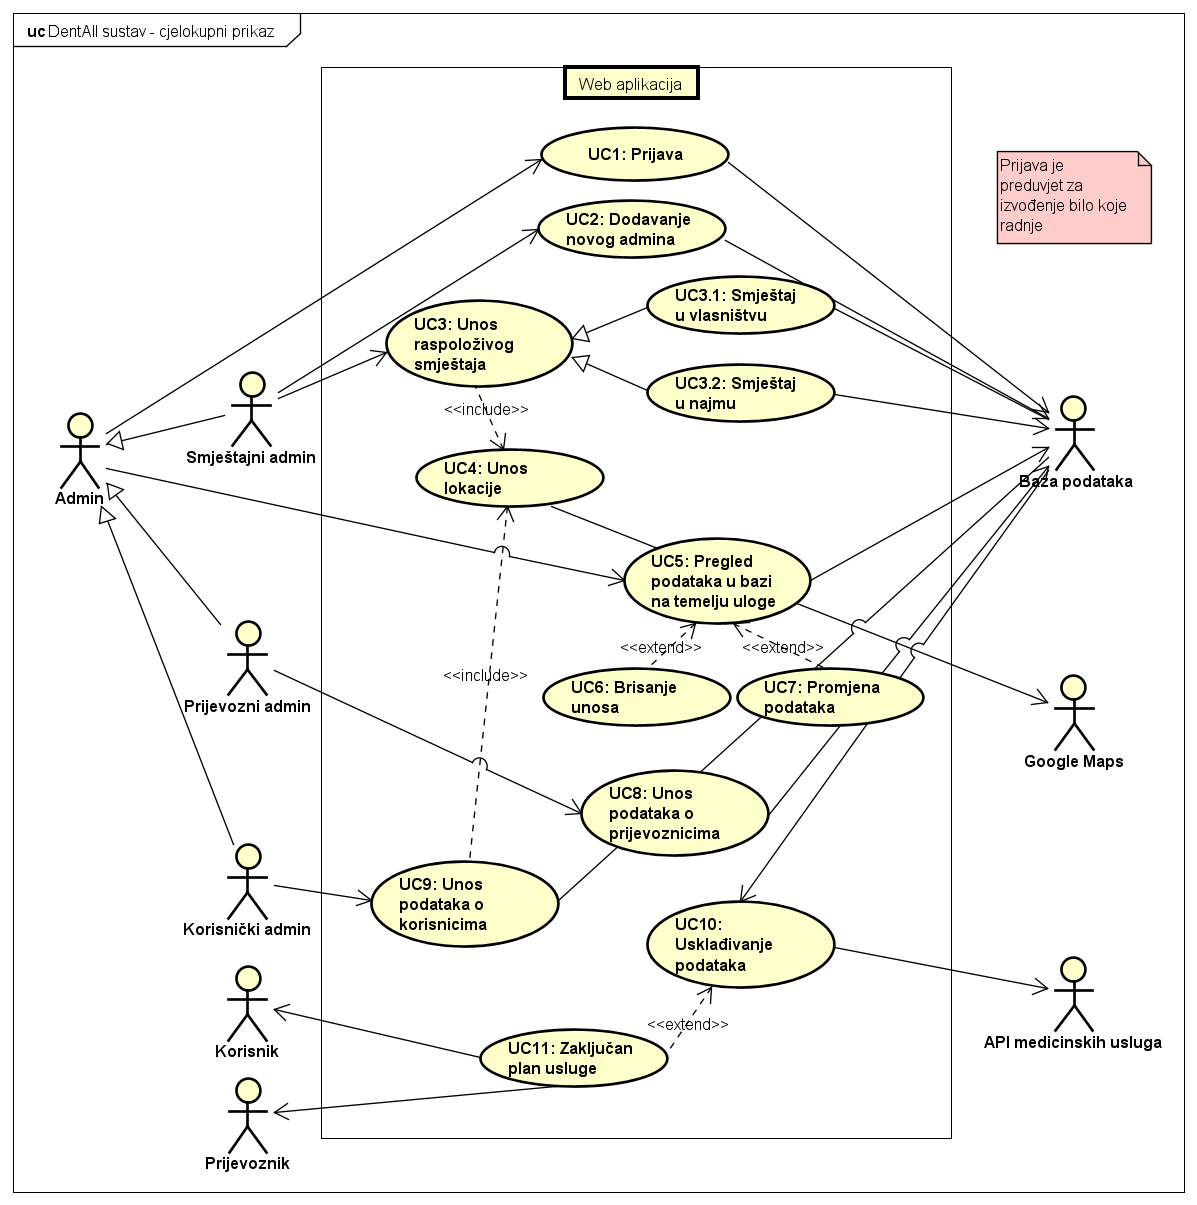
\includegraphics[width=\linewidth]{slike/Cjelokupni-prikaz-1.PNG} 
					\centering
					\caption{Sveobuhvatni prikaz}
					\label{fig:sveobuhvatniPrikaz}
				\end{figure}
				
				\begin{figure}[H]
					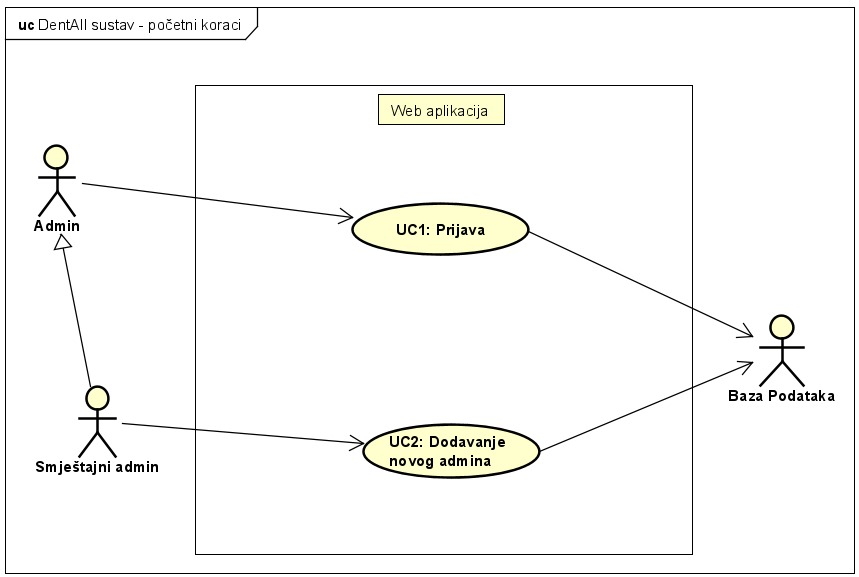
\includegraphics[width=\linewidth]{slike/DentAll_Pocetni-Koraci.PNG} 
					\centering
					\caption{Početni koraci}
					\label{fig:pocetniKoraci}
				\end{figure}
				
				\begin{figure}[H]
					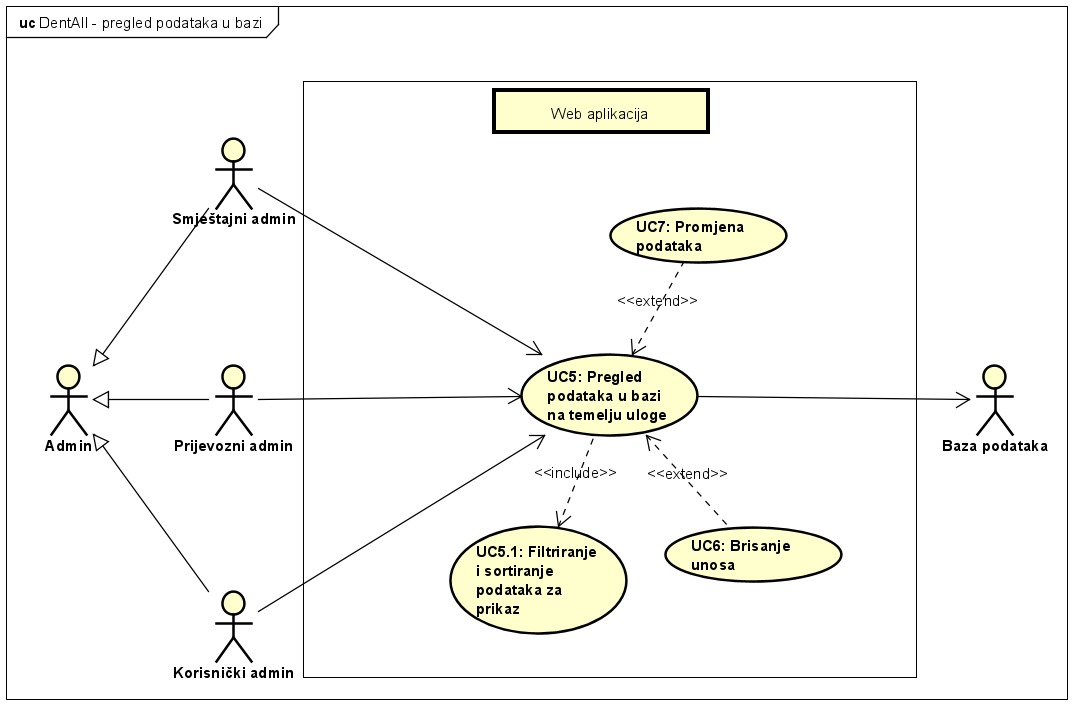
\includegraphics[width=\linewidth]{slike/DentAll_PregledPodatakaUBazi.PNG}
					\centering
					\caption{Pregled podataka u bazi podataka}
					\label{fig:pregledPodataka}
				\end{figure}
				
				\begin{figure}[H]
					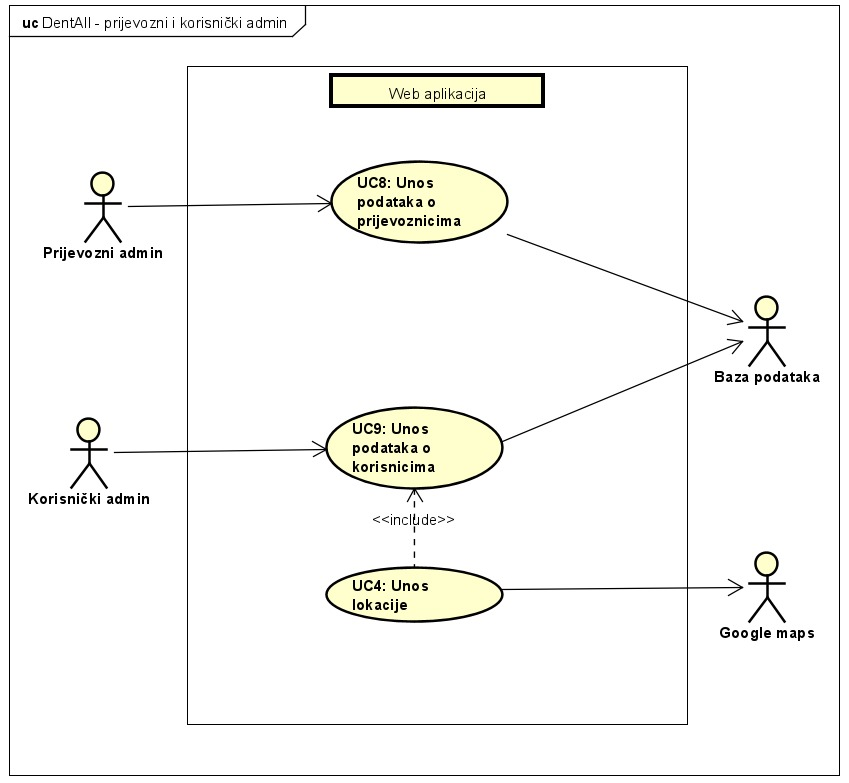
\includegraphics[width=\linewidth]{slike/DentAll_PrijevozniIKorisničkiAdmin.png}
					\centering
					\caption{Prikaz uloga korisničkog i prijevoznog administratora}
					\label{fig:prijevozniIKorisničkiAdmin}
				\end{figure}
				
				\begin{figure}[H]
					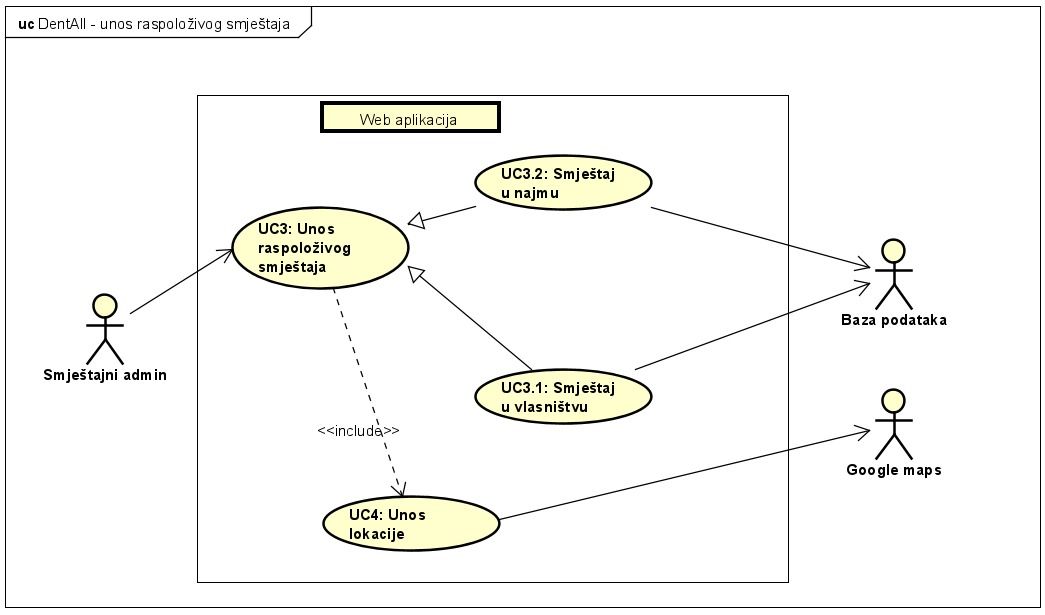
\includegraphics[width=\linewidth]{slike/DentAll_UnosRaspoloživogSmještaja.png} 
					\centering
					\caption{Prikaz unosa raspooloživog smještaja}
					\label{fig:unosSmještaja}
				\end{figure}
				
				\begin{figure}[H]
					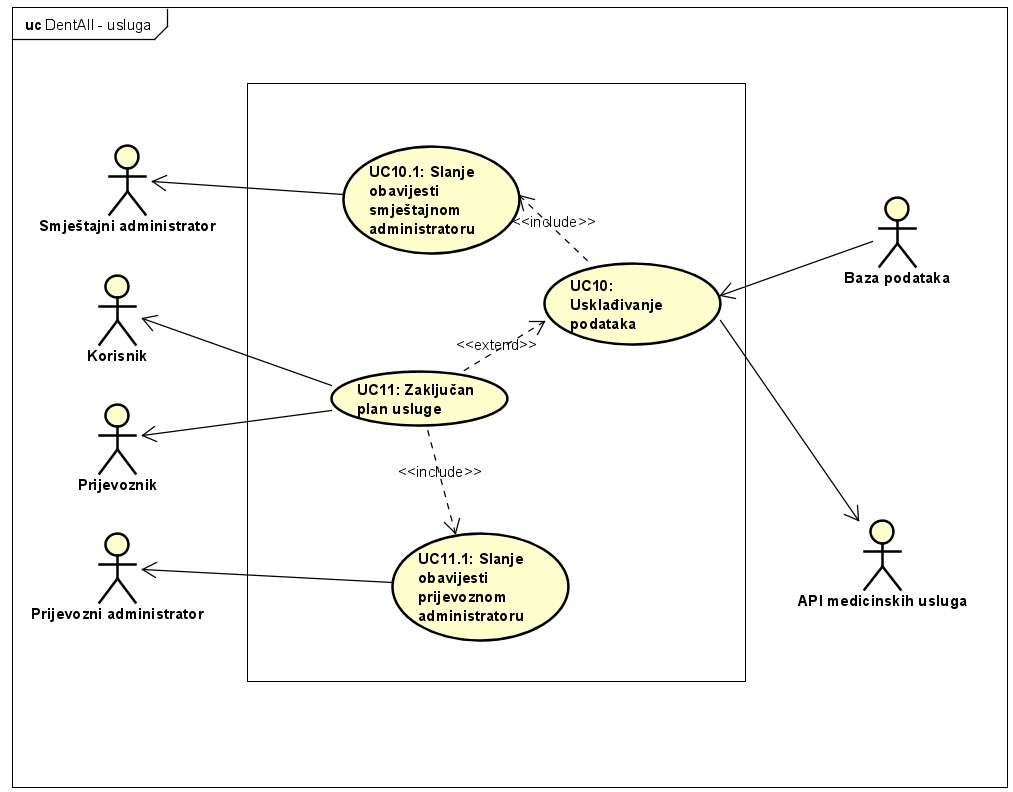
\includegraphics[width=\linewidth]{slike/DentAll_Usluga.png}
					\centering
					\caption{Prikaz korisničke strane}
					\label{fig:korisnik}
				\end{figure}
				
			\subsection{Sekvencijski dijagrami}
				
				\textbf{\textit{dio 1. revizije}}\\
				\texbf{UC1-Prijava}
				{Administrator unosi korisničko ime i lozinku.Web preglednik to upućuje bazi podataka na validaciju. Ako korisnički podaci nisu ispravni ili su nepoznati, korisnikova prijava nije uspjela te se ispisuje greška. Ako je prijava uspjela korisnik je preusmjeren na početnu stranicu.}
				
				\begin{figure}[H]
					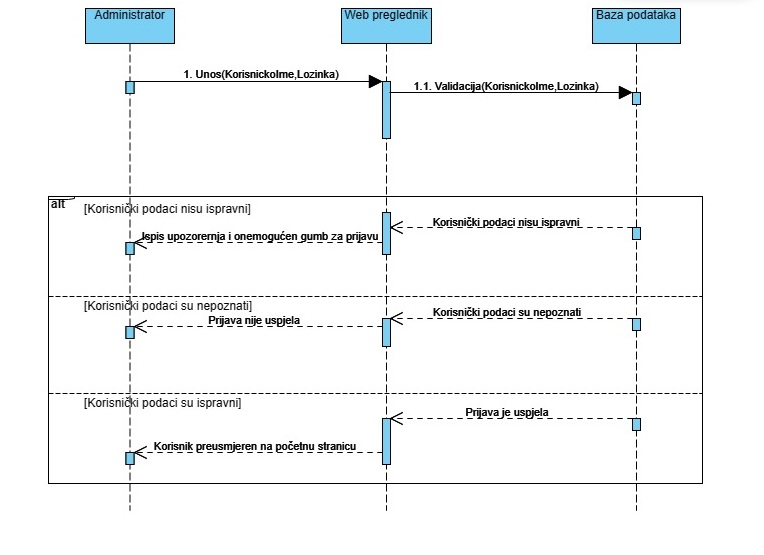
\includegraphics[width=\linewidth]{slike/DentAll_Sekvencijski-UC1-Prijava.jpeg} 
					\centering
					\caption{Sekvencijski dijagram UC1-Prijava}
					\label{fig:Sekvencijski dijagram UC1}
				\end{figure}
				
				\newpage
				
					\texbf{UC2-Dodavanje novog administratora}
					
					{Smještajni administrator prvo se mora prijaviti (UC1-Prijava). Nakon toga odabire opciju za dodavanje novog korisnika te upisuje njegove podatke. Dok nije unesen korisnik u dobrom formatu, korisniku (smještajnom administratoru) se ispisuje upozorenje o krivom formatu. Nakon što se unese dobar format, smještajni administrator unosi ulogu. Dok nije označena uloga ispisuje se upozorenje o neoznačenoj ulozi. Nakon što je uloga označena, smještajni administrator moram kliknuti na gumb pri čemu se šalje zahtjev za unos u bazu podataka. Baza  podataka može vratiti grešku te se ispisuje poruka o grešci korisniku ili se može ponovno poslati zahtjev za unos u bazu podataka. Nakon što je korisnik uspješno unesen, smještajnom administratoru se sva polja vračaju na početnu vrijednost.}
				
				\begin{figure}[H]
					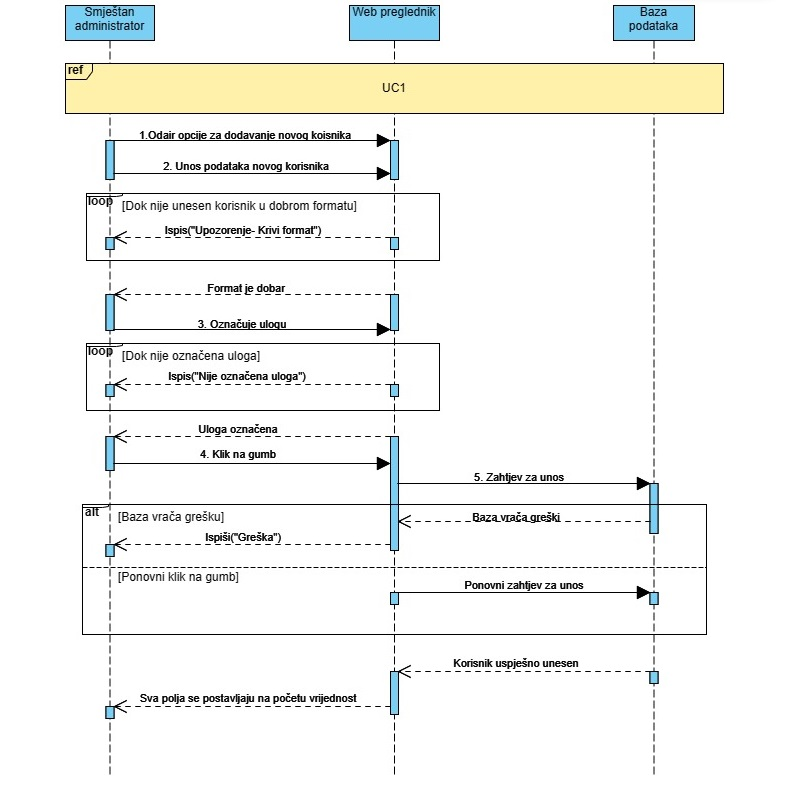
\includegraphics[width=\linewidth]{slike/DentAll-Sekvencijski-uc2-Dodavanje_novog_administratora.jpeg}
					\centering
					\caption{Sekvencijski dijagram UC2-Dodavanje novog administratora}
					\label{fig:Sekvencijski dijagram UC2}
				\end{figure}
				
				\newpage
				
				
				\texbf{UC3-Unos razpoloživog smještaja}
				
				{Smještajni administrator se prvo se mora prijaviti(UC1-Prijava). Nakon toga smještajni administrator odabire opciju dodavanja novog smještaja te odabire tip stana. Web preglednik pošalje zahtjev bazi podataka za unos te baza ako nije odabran tip šalje povratnu informaciju pregledniku, a preglednik korisniku ispiše upozorenje o odabiru tipa. Ako je uspješno odabran tip , sljedeće se unosi kategorija, te ponovno šalje zahtjev za unos, ako nije odabrana kategorija ispisuje se upozorenje o odabiru kategorije. Nakon što je kategorija uspješno odabrana, smještajni administrator odabire maksimalan kapacitet i unosi informacije o zgradi,web preglednik ponovno pošalje zahtjev za unos, te baza podataka može poslati grešku nazad u slučaju ako je krivi format unosa. Na kraju smještajni administrator odabire tip vlasništva, čime se detaljnije bave UC3.1 -Smještaj u vlasništvu i UC3.2 - Smještaj u najmu.}
				
				\begin{figure}[H]
					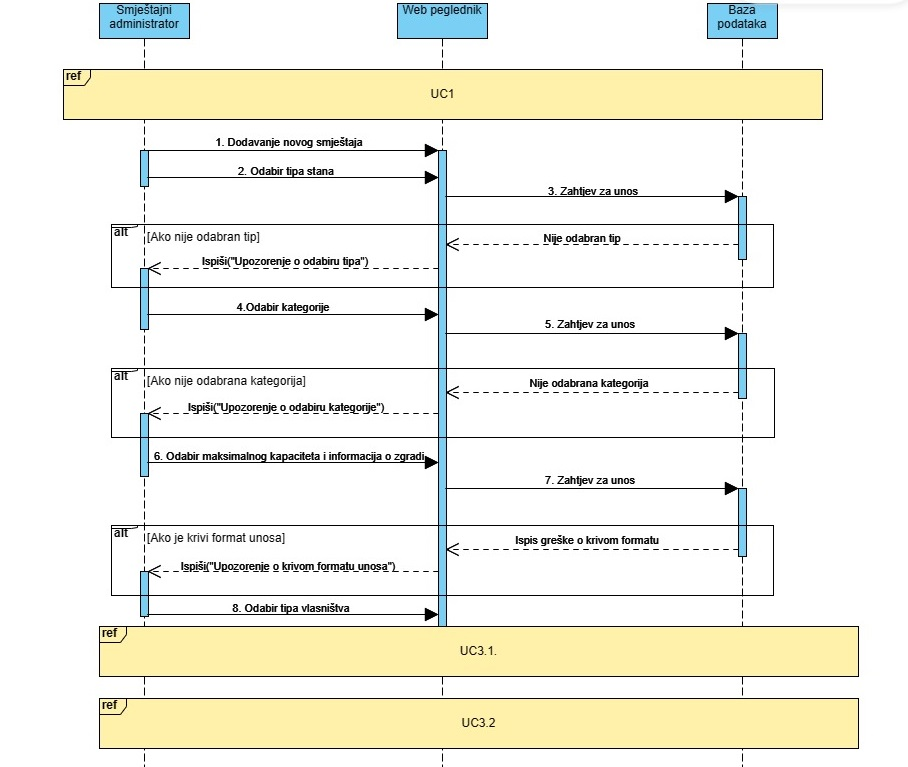
\includegraphics[width=\linewidth]{slike/DentAll-Sekvencijski-uc3-unos_raspoloživog_smještaja.jpg}
					\centering
					\caption{Sekvencijski dijagram UC3-Unos raspoloživog smještaja}
					\label{fig:Sekvencijski dijagram UC3}
				\end{figure}
				
				\eject
	
		\section{Ostali zahtjevi}
		
			\textbf{\textit{dio 1. revizije}}\\
		 
			 \textit{Nefunkcionalni zahtjevi i zahtjevi domene primjene dopunjuju funkcionalne zahtjeve. Oni opisuju \textbf{kako se sustav treba ponašati} i koja \textbf{ograničenja} treba poštivati (performanse, korisničko iskustvo, pouzdanost, standardi kvalitete, sigurnost...). Primjeri takvih zahtjeva u Vašem projektu mogu biti: podržani jezici korisničkog sučelja, vrijeme odziva, najveći mogući podržani broj korisnika, podržane web/mobilne platforme, razina zaštite (protokoli komunikacije, kriptiranje...)... Svaki takav zahtjev potrebno je navesti u jednoj ili dvije rečenice.}
			 \begin{packed_item}
                \item Aplikacija mora biti u mogućnosti grafički prikazati geografski položaj nekretnine korištenjem Google Maps/Open Maps usluge.
                \item Aplikacijsko sučelje mora imati mogućnost preuzimanja detalja korisnikovih tretmana iz aplikacije za evidenciju medicinskih usluga.
                \item Sustav treba biti jednostavan za korištenje.
                \item Korištenje sustava ne smije narušavati njegovu funkcionalnost i rad.
                \item Svi privatni podatci u sustavu moraju biti zaštićeni.
                \item Lozinke moraju biti sigurno spremljene u bazi.
                \item Nadogradnja sustava ne smije narušavati njegove postojeće funkcije.
                \item Sustav treba podržavati istovremeni rad više korisnika.
		  	\end{packed_item}
			 
			 
	
	\chapter{Arhitektura i dizajn sustava}
		
		%\textbf{\textit{dio 1. revizije}}\\

		%\textit{ Potrebno je opisati stil arhitekture te identificirati: podsustave, preslikavanje na radnu platformu, spremišta podataka, mrežne protokole, globalni upravljački tok i sklopovsko-programske zahtjeve. Po točkama razraditi i popratiti odgovarajućim skicama:}
	\begin{itemize}
		\item 	%\textit{izbor arhitekture temeljem principa oblikovanja pokazanih na predavanjima (objasniti zašto ste baš odabrali takvu arhitekturu)}
		Aplikacija se sastoji od backend-a, frontend-a i baze podataka. \newline Backend je pozadinski dio aplikacije koji se izvršava na serveru. Za razvoj backend-a odabran je programski jezik Java i okvir Spring što čini backend prenosiv i jednostavan za korištenje. Sastoji se od rest kontrolera koji primaju HTTP zahtjeve i vraćaju JSON podatke, Service komponenti koje provjeravaju točnost upita i valjanost njihovih vrijednosti te konačno Repository komponenti koji omogućuju upisivanje u bazu i čitanje iste. \newline Frontend je grafičko sučelje koje omogućuje prijavu u aplikaciju, prikaz traženih podataka te lakše korištenje aplikacije. Za razvoj frontend-a odabran je programski jezik TypeScript u kojem je korišten React te React router biblioteka. Taj odabir omogućuje razvoj stranice uz pomoć tzv. komponenti što čini kod čitljivije i dopušta lakše ponovno korištenje. Za izgled stranice korišten je Bootstrap kako bi stranica imala moderan izgled. \newline Baza podataka pisana je u programskom jeziku SQL zbog njegove široke upotrebe i visoke kompatibilnosti.
		\item	%\textit{organizaciju sustava s najviše razine apstrakcije (npr. klijent-poslužitelj, baza podataka, datotečni sustav, grafičko sučelje)}
		Ulaskom na aplikaciju korisnik (administrator) je preusmjeren na stranicu za prijavu. Nakon unosa svog korisničkog imena i lozinke, podatci se provjeravaju, i ako su ispravni, administratora se preusmjerava na administratorsku stranicu. Ondje su prikazani različiti podaci ovisno o tome koji administrator pristupa stranici, na primjer smještajni administrator vidi samo podatke vezane uz smještaj. \newline Sustav dodatno komunicira sa vanjskim API-em kako bi dobio podatke koje mu trebaju te ih zatim sprema u bazu podataka iz koje ih dobavlja svaki sljedeći put. 
		\item 
		Frontend je organiziran u jednoj mapi (\textit{IzvorniKod/error404-fe/error404}) te dvije podmape, u mapi se nalaze paketi i dodaci potrebni za pokretanje frontend-a te podmape \textit{src} i \textit{public}. Unutar podmape \textit{src} nalazi se sam kod frontend dijela aplikacije te u mapama \textit{assets} i \textit{components} se redom nalaze \textit{namespace} u .svg obliku, te dodatne komponente koje omogućavaju rad frontend-a. \newline Backend je organiziran u jednoj mapi (\textit{IzvorniKod/error404-be}), te dvije podmape, \textit{src} i \textit{docker}. U mapi \textit{src/main} nalazi se sav kod za backend, on je podjeljen u dvije podmape. Unutar mape \textit{java/dentall} nalazi se kod koji je pisan u programskom jeziku Javi, on je podjeljen na više podmapa u kojima se nalaze dijelovi MVC arhitekture, u mapi \textit{dao} nalaze se Repository komponente koji služi dohvaćanju podataka iz baze, u mapi \textit{service} nalaze se Service komponenete, u mapi \textit{rest} nalaze se kontroleri, u mapi \textit{domain} nalaze se ostale klase koje sadrže objektne reprezentacije podataka iz baze. Unutar mape \textit{resources} nalazi se mapa baza podataka \textit{db} koja se sastoji od 2 podmape \textit{sql} i \textit{changelog}, gdje se redom nalaze sam SQL kod baze podataka te datoteke pisane u XML-u (\textit{eXtensive Markup Language}) koje služe boljem povezivanju baze podataka sa backend-om. U mapi \textit{docker} nalazi se \textit{Dockerfile} koji sadrži programski kod potreban za izgradnju (\textit{build}) same aplikacije.
		
		
	\end{itemize}
		\section{Baza podataka}
			
			%\textbf{\textit{dio 1. revizije}}\\
			
		%\textit{Potrebno je opisati koju vrstu i implementaciju baze podataka ste odabrali, glavne komponente od kojih se sastoji i slično.}\\
		
		{Baza podataka modelirana je tabličnim modelom u "\textit{Structured Query Language}" (SQL) jeziku. Ona se sastoji od osam entiteta. Entiteti baze podataka su tablice u kojima su zadržani podaci potrebni za rad cijelog sustava. Tablice su redom \textbf{Korisnik}, \textbf{Smještaj}, \textbf{Adresa}, \textbf{Vozilo}, \textbf{Vozač}, \textbf{Admin}, \textbf{AdminUloga} i \textbf{Uloge}. Unutar baze je moguće dodavati (\textit{insert}), mijenjati (\textit{update}) i brisati (\textit{delete}) podatke koje ona sadrži, također je moguće izvršavati \textit{select} i agregatne upite koji će prikazivati traženi sadržaj koji se nalazi unutar baze podataka.}
		
			\subsection{Opis tablica}
			
				
				{Entitet \textbf{Korisnik} sadržava informacije o korisniku. Atributi od kojih se sastoji entitet su: IDKor koji je ujedno i identifikacijski ključ korisnika,
				Ime, Prezime, DatDol odnosno vrijeme dolaska, DatOdl vrijeme odlaska, IdSmj, RegVoz i OdvoziRez. Ovaj entitet je u vezi One-to-One s entitetom  Smještaj preko atibuta
				IDSmj, te je u vezi One-to-One s entitetom Vozilo preko atributa RegVoz i OdlaziRegVoz.}
				
				\begin{longtblr}[
					label=none,
					entry=none
					]{
						width = \textwidth,
						colspec={|X[6,l]|X[6, l]|X[20, l]|}, 
						rowhead = 1,
					} %definicija širine tablice, širine stupaca, poravnanje i broja redaka naslova tablice
					\hline \SetCell[c=3]{c}{\textbf{Korisnik}}	 \\ \hline[3pt]
					\SetCell{LightGreen}IDKor & INT	&  	Identifikacijski ključ korinika	\\ \hline
					Ime	& VARCHAR & Ime korisnika  	\\ \hline 
					Prezime & VARCHAR &  Prezime korisnika \\ \hline 
					DatDol & TIMESTAMP	&  Datum dolaska korisnika		\\ \hline 
					DatOdl & TIMESTAMP	&  Datum odlaska korisnika		\\ \hline 
					\SetCell{LightBlue}IdSmj & INT	&  Identifikacijski ključ smještaja		\\ \hline 
					\SetCell{LightBlue}RegVozila & VARCHAR	& Identifikacijski ključ vozila u dolasku		\\ \hline 
					\SetCell{LightBlue}OdvoziReg	& VARCHAR & Identifikacijski ključ vozila u odlasku 	\\ \hline 
				\end{longtblr}
				
				{Entitet \textbf{Smještaj} opisuje smještaj u kojem će boraviti korisik. Sadrži atribute: IDSmj (ujedno i identifikacijski ključ), vrsta smještaja te IDAdr. Entitet Smještaj povezan je sa
				vezom Many-to-Many s entitetom Adresa preko	atributa IDAdr.}
				
				\begin{longtblr}[
					label=none,
					entry=none
					]{
						width = \textwidth,
						colspec={|X[6,l]|X[6, l]|X[20, l]|}, 
						rowhead = 1,
					} %definicija širine tablice, širine stupaca, poravnanje i broja redaka naslova tablice
					\hline \SetCell[c=3]{c}{\textbf{Smještaj}}	 \\ \hline[3pt]
					\SetCell{LightGreen}IDSmj & INT	&  	Identifikacijski ključ smještaja	\\ \hline
					Vrsta	& VARCHAR & Vrsta smještaja  	\\ \hline 
					\SetCell{LightBlue}IDAdr	& INT & Identifikacijski ključ adrese smještaja 	\\ \hline 
				\end{longtblr}
				
				{Entitet \textbf{Adresa} govori o samoj adresi smještaja i to s atributima: IDAdr, Mjesto, Ulica i Broj. Identifikacijski ključ ovog entiteta je IDAdr.}
				
				\begin{longtblr}[
					label=none,
					entry=none
					]{
						width = \textwidth,
						colspec={|X[6,l]|X[6, l]|X[20, l]|}, 
						rowhead = 1,
					} %definicija širine tablice, širine stupaca, poravnanje i broja redaka naslova tablice
					\hline \SetCell[c=3]{c}{\textbf{Adresa}}	 \\ \hline[3pt]
					\SetCell{LightGreen}IDAdr & INT	&  	Identifikacijski ključ adrese	\\ \hline
					Mjesto	& VARCHAR & Mjesto u adresi smještaja	\\ \hline 
					Ulica	& VARCHAR & Ulica u adresi smještaja	\\ \hline 
					Broj	& INT & Kućni broj u adresi smještaja	\\ \hline  
				\end{longtblr}


				{Entitet \textbf{Vozilo} sadrži informacije o samom vozilu. Sadrži atribute: RegVozila (registracija vozila), Model i Boja. Identifikacijski ključ entiteta je registracija vzila (RegVoz)}
				
				\begin{longtblr}[
					label=none,
					entry=none
					]{
						width = \textwidth,
						colspec={|X[6,l]|X[6, l]|X[20, l]|}, 
						rowhead = 1,
					} %definicija širine tablice, širine stupaca, poravnanje i broja redaka naslova tablice
					\hline \SetCell[c=3]{c}{\textbf{Vozilo}}	 \\ \hline[3pt]
					\SetCell{LightGreen}RegVozila & VARCHAR	&  	Identifikacijski ključ vozila	\\ \hline
					Model	& VARCHAR & Model vozila	\\ \hline 
					Boja	& VARCHAR & Boja vozila	\\ \hline 
				\end{longtblr}

				{Entitet \textbf{Vozač} opisuje vozača koji vozi i odvozi korisnika u i iz njegovog privremenog smještaja. Sadrži atribute: IDVoz (identifikacijski ključ), Ime, Prezime, Brradsat(broj radnih sati) te Regvozila. Povezan je s entitetom Vozilo sa vezom Many-to-Many preko atributa RegVozila.}
				
				\begin{longtblr}[
					label=none,
					entry=none
					]{
						width = \textwidth,
						colspec={|X[6,l]|X[6, l]|X[20, l]|}, 
						rowhead = 1,
					} %definicija širine tablice, širine stupaca, poravnanje i broja redaka naslova tablice
					\hline \SetCell[c=3]{c}{\textbf{Vozač}}	 \\ \hline[3pt]
					\SetCell{LightGreen}IDVoz & INT	&  	Identifikacijski ključ vožača	\\ \hline
					Ime	& VARCHAR & Ime vozača	\\ \hline 
					Prezime	& VARCHAR & Prezime vozača	\\ \hline
					Brradsat	& INT & Broj radnih sati vozača	\\ \hline  
					\SetCell{LightBlue}RegVozila	& VARCHAR & Identifikacijski ključ vozila 	\\ \hline
				\end{longtblr}

				{Entitet \textbf{Admin} sadrži informacije o adminu profilu te se sastoji od artibuta: UserName i lozinka.}
				
				\begin{longtblr}[
					label=none,
					entry=none
					]{
						width = \textwidth,
						colspec={|X[6,l]|X[6, l]|X[20, l]|}, 
						rowhead = 1,
					} %definicija širine tablice, širine stupaca, poravnanje i broja redaka naslova tablice
					\hline \SetCell[c=3]{c}{\textbf{Admin}}	 \\ \hline[3pt]
					\SetCell{LightGreen}UserName & VARCHAR	&  	Identifikacijski ključ admina	\\ \hline
					Lozinka	& VARCHAR & Lozinka admina	\\ \hline 
					\end{longtblr}
			
				{Entitet \textbf{AdminUloga} povezuje admina s njegovom ulogom. Sastoji se od atributa: UserName i IDUloge. Povezan je s entitetom Admin s vezom Many-to-Many te preko atributa UserName, te je spojen također s vezom Many-to-Many s entiteom Uloge preko atributa IDUloge.}
				
				\begin{longtblr}[
					label=none,
					entry=none
					]{
						width = \textwidth,
						colspec={|X[6,l]|X[6, l]|X[20, l]|}, 
						rowhead = 1,
					} %definicija širine tablice, širine stupaca, poravnanje i broja redaka naslova tablice
					\hline \SetCell[c=3]{c}{\textbf{AdminUloga}}	 \\ \hline[3pt]
					\SetCell{LightBlue}UserName	& VARCHAR & Orisničko ime admina 	\\ \hline
					\SetCell{LightBlue}IDUloge	& VARCHAR & ID Uloge admina	\\ \hline
					\end{longtblr}

				{Entitet \textbf{Uloge} sadrži informacije o samoj ulozi. Aributi od kojij se sastoji su: IDUloge(identifikacijski ključ) te Uloga}
				
				\begin{longtblr}[
					label=none,
					entry=none
					]{
						width = \textwidth,
						colspec={|X[6,l]|X[6, l]|X[20, l]|}, 
						rowhead = 1,
					} %definicija širine tablice, širine stupaca, poravnanje i broja redaka naslova tablice
					\hline \SetCell[c=3]{c}{\textbf{Uloge}}	 \\ \hline[3pt]
					\SetCell{LightGreen}IDUloge & VARCHAR	&  	Identifikacijski ključ uloge admina	\\ \hline
					Uloga	& VARCHAR & Uloga admina	\\ \hline 
					\end{longtblr}

			\subsection{Dijagram baze podataka}
				%\textit{ U ovom potpoglavlju potrebno je umetnuti dijagram baze podataka. Primarni i strani ključevi moraju biti označeni, a tablice povezane. Bazu podataka je potrebno normalizirati. Podsjetite se kolegija "Baze podataka".}
			
			
			\begin{figure}[H]
				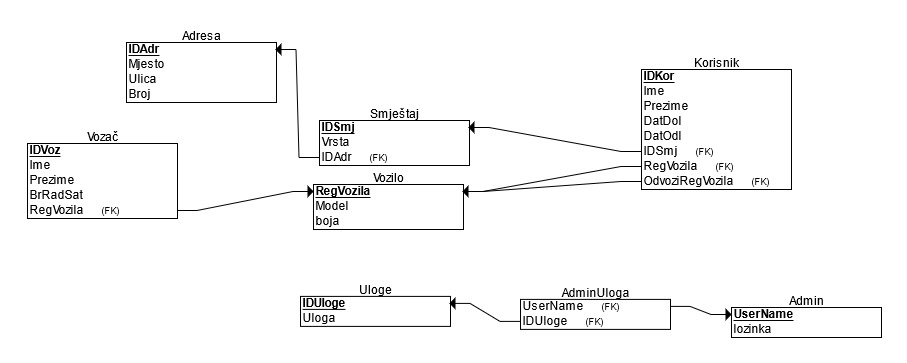
\includegraphics[width=\linewidth]{slike/DentAll_RelacijskiDijagramBaze.png}
				\centering
				\caption{Dijagram baze podataka}
				\label{fig:dijagramBaze}
			\end{figure}
			\eject
			
		\section{Dijagram razreda}
		
			{Na sljedećim slikama prikazani su dijagrami razreda koji se odnose na \textit{backend} dio aplikacije. Na slici 4.1 prikazan je cjelokupni dijagram razreda, a na ostalima su razdvojeni u smislene cjeline. U implementaciji korištena je \textit{Spring Boot} tehnologija. Postoje tri sloja aplikacije: \textit{Controller}(REST API), \textit{Service}(poslovna logika) te \textit{Repository}(pristup podacima). }\\
			
			\begin{figure}[H]
				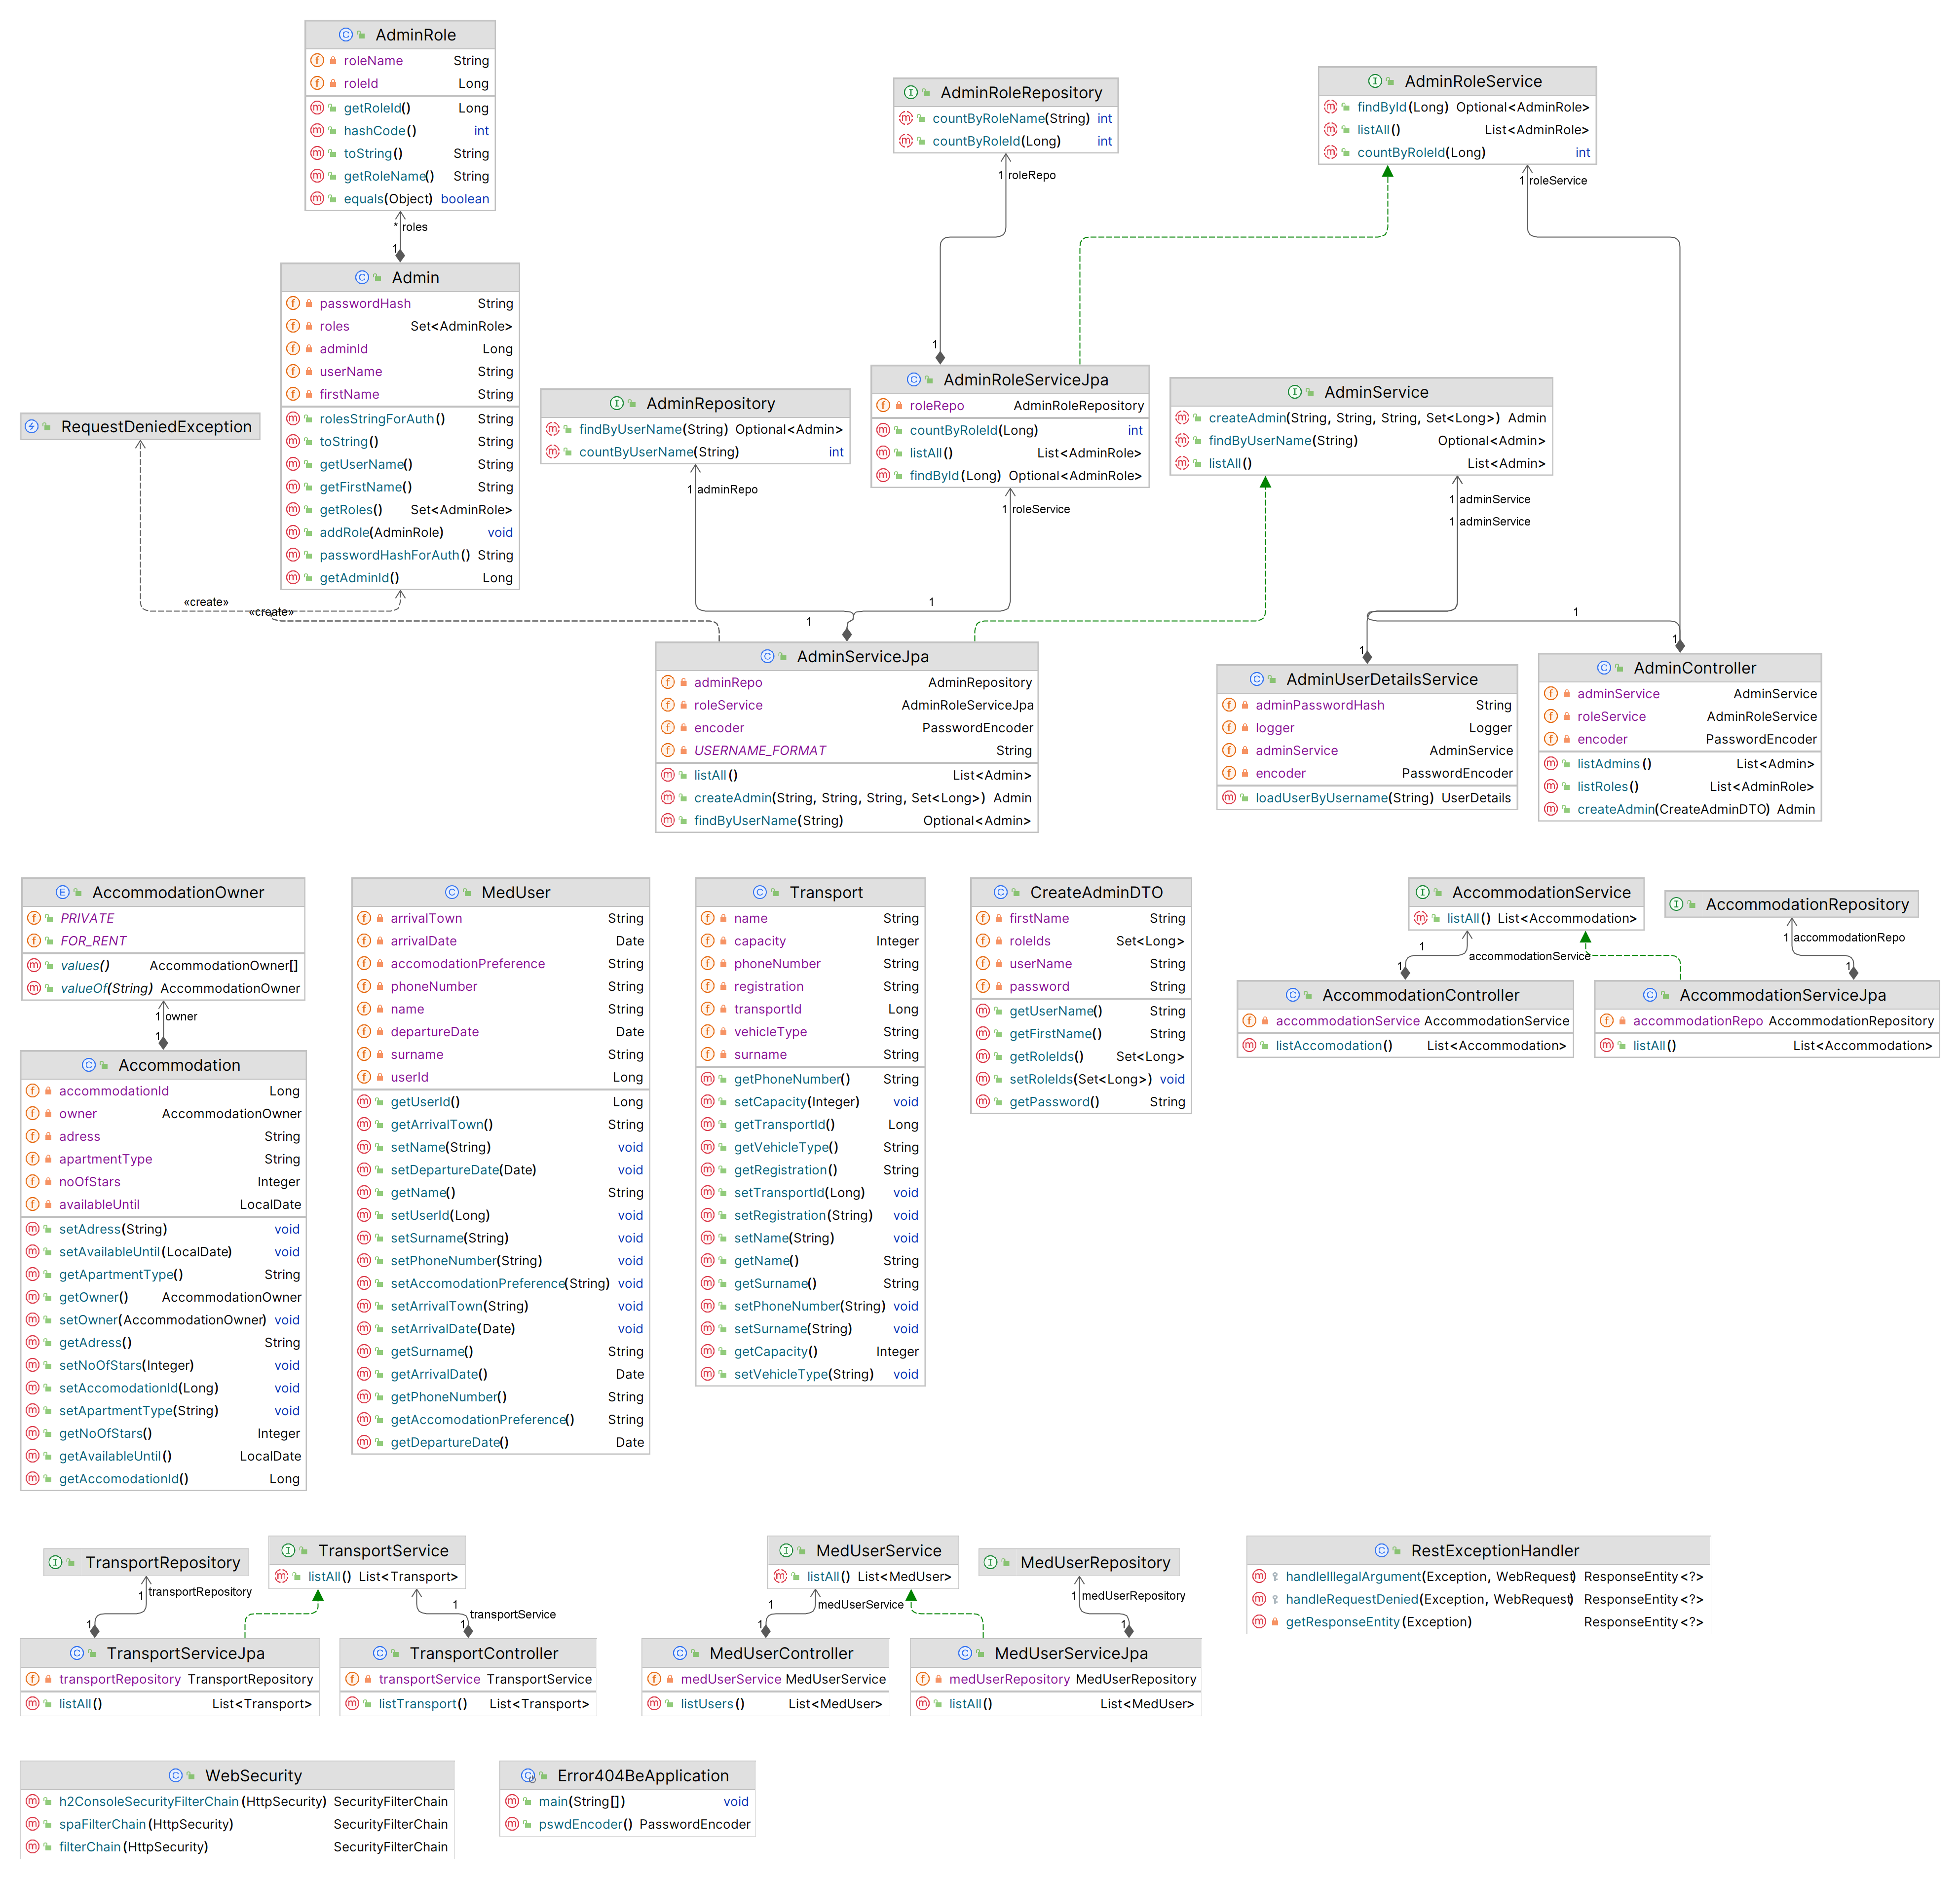
\includegraphics[width=\textwidth]{slike/CjelokupanDijagramRazreda.PNG}
				\caption{Cjelokupan dijagram razreda}
				\label{classDiagram}
			\end{figure}
			
			\begin{figure}[H]
				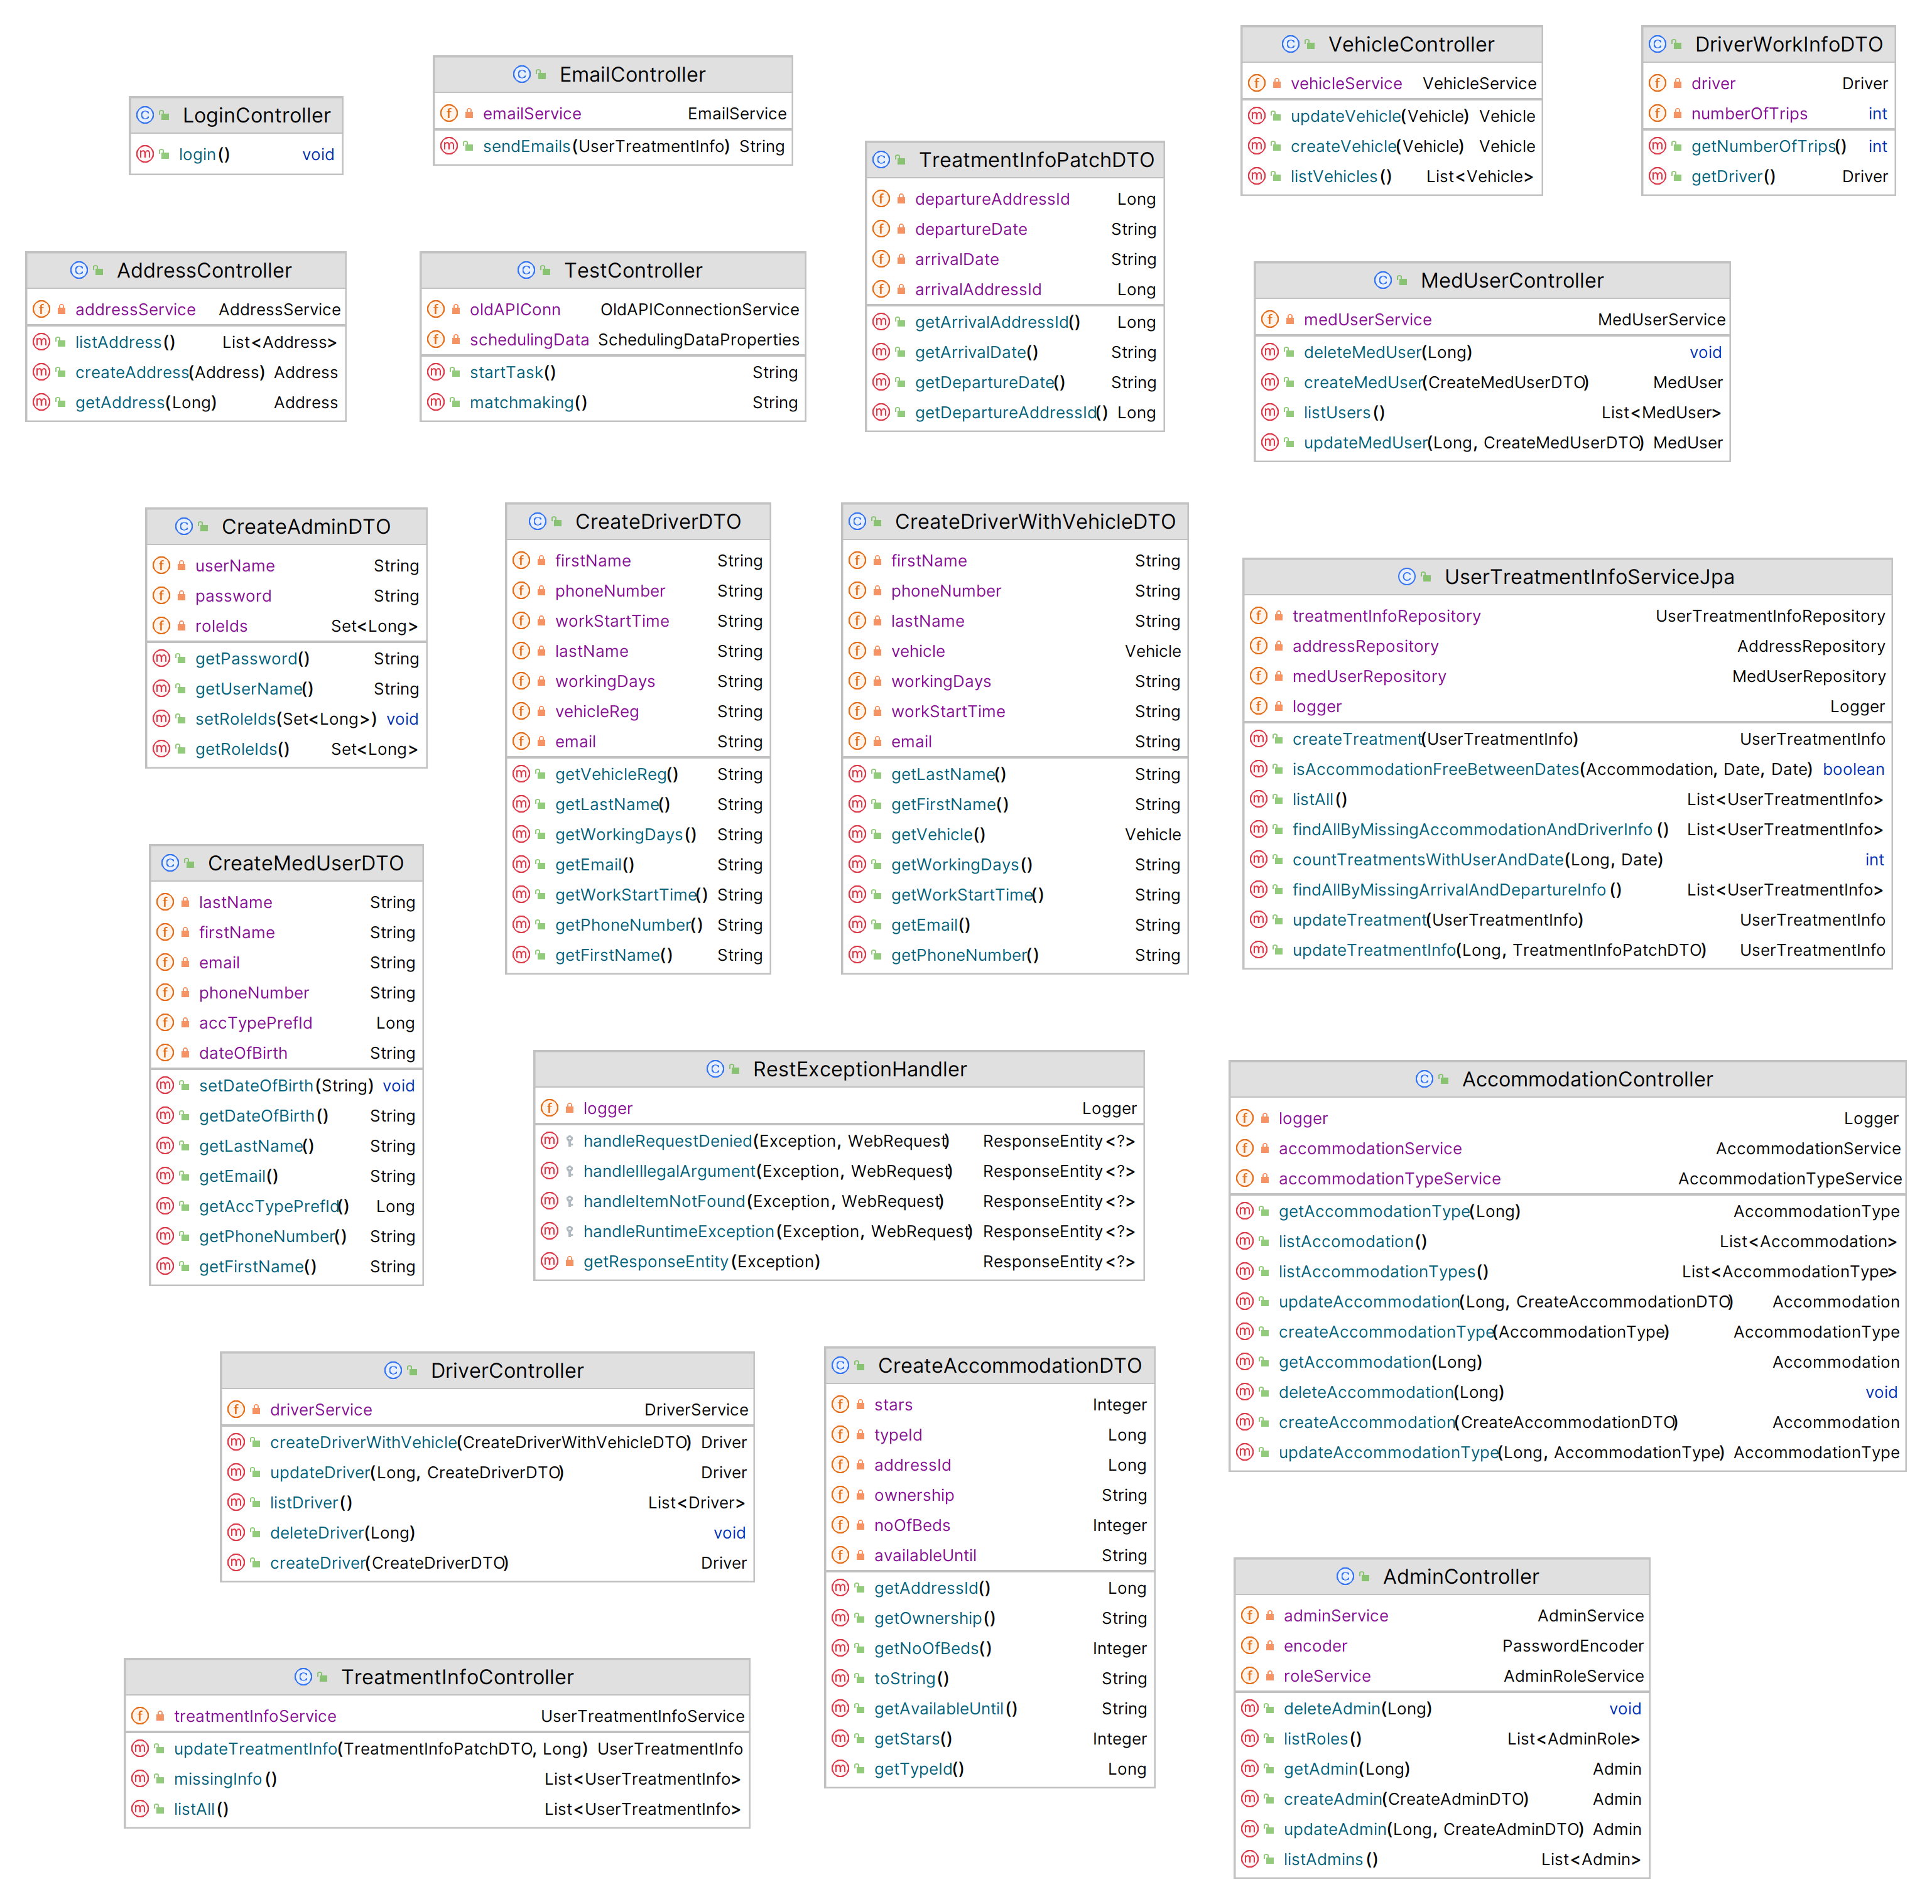
\includegraphics[width=\textwidth]{slike/rest.PNG}
				\caption{Dijagram razreda - Controller}
				\label{restDiagram}
			\end{figure}
			
			{Navedene klase nasljeđuju REST Controller koji je zadužen za rukovanje HTTP zahtjevima i za pružanje odgovarajućih odgovora. REST Controller vraća podatke u JSON formatu. \\ 
			CreateAdminDTO je \textit{Data transfer Object} koji je zadužen za stvaranje administratora. \textit{DTO} služi za transfer podataka između slojeva aplikacije, pogotovo između klijenta i servera. \\
			AdminUserDetailsService je \textit{Spring service} komponenta koja služi za baratanje detaljima administratora tijekom prijave i prilagođavanje korisničkih detalja na temelju odgovarajućih uloga i vjerodajnica, te osiguravanje sigurnosti}\\
			
			\begin{figure}[H]
				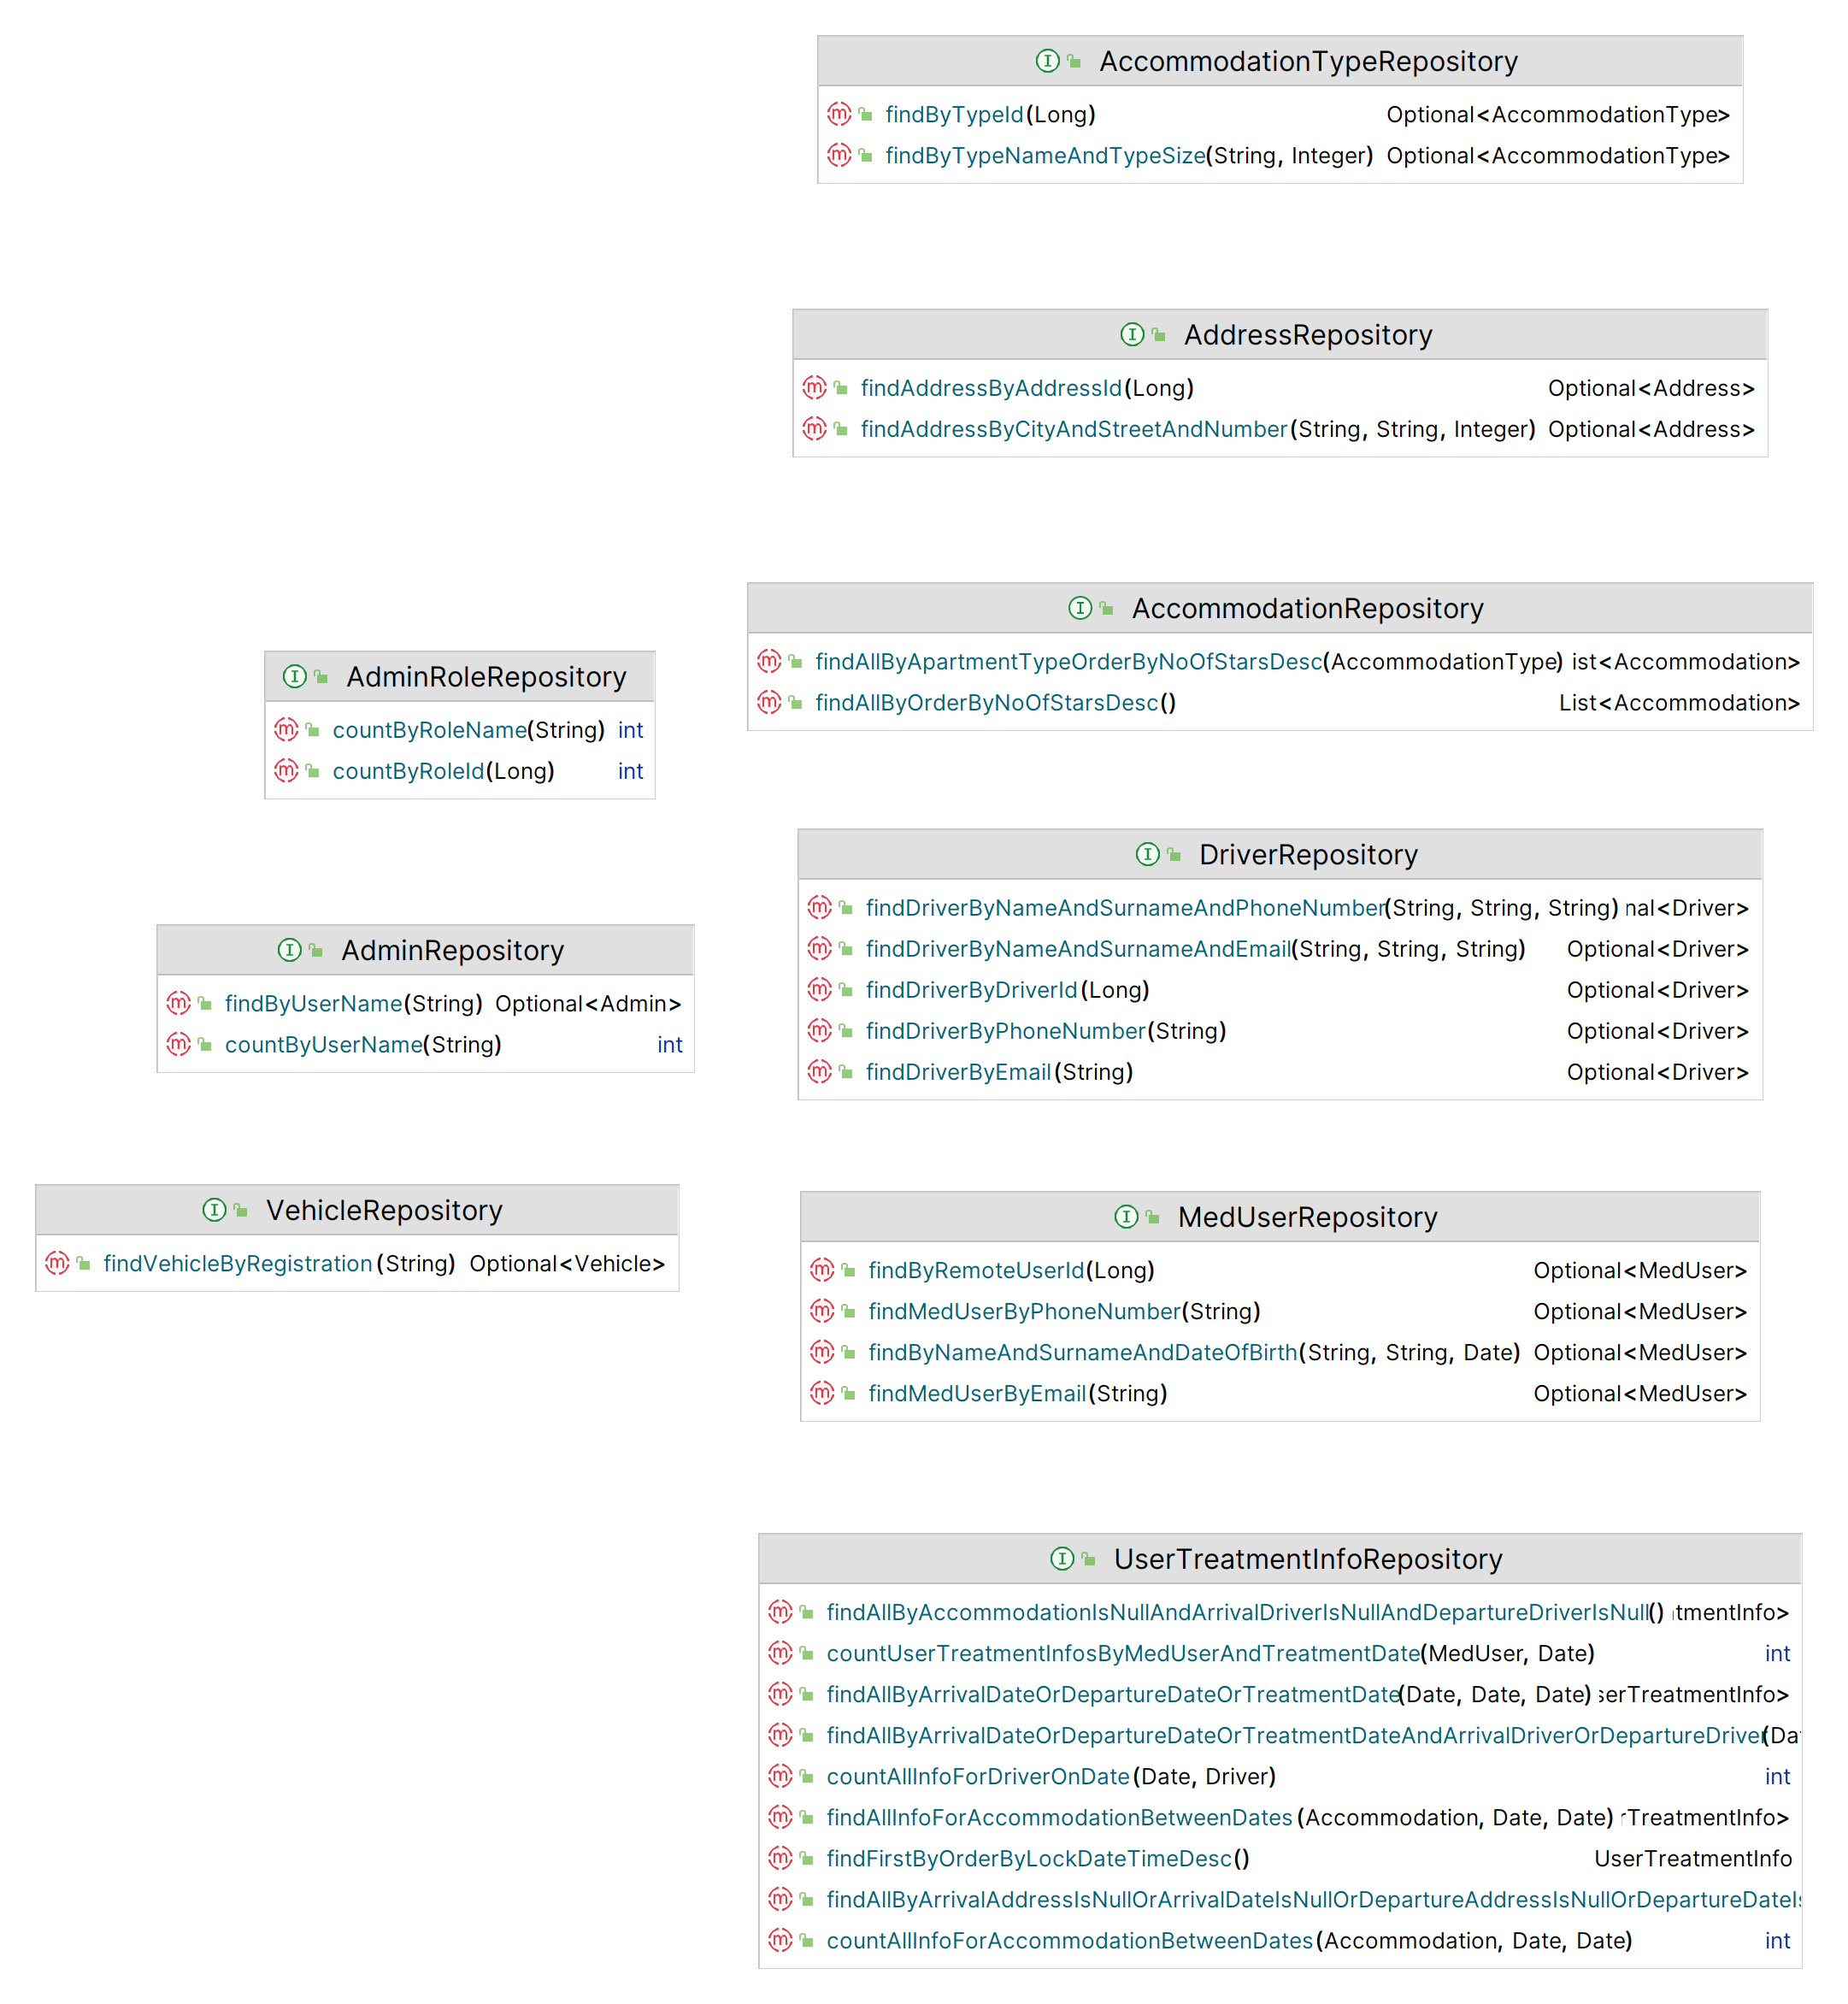
\includegraphics[width=\textwidth]{slike/dao.PNG}
				\caption{Dijagram razreda - Repository}
				\label{repositoryDiagram}
			\end{figure}
			
			{Navedena sučelja nasljeđuju \textit{JPARepository} koji pruža generičke metode za operacije s podatcima, poput spremanja, ažuriranja, brisanja i slično.}\\
			
			\begin{figure}[H]
				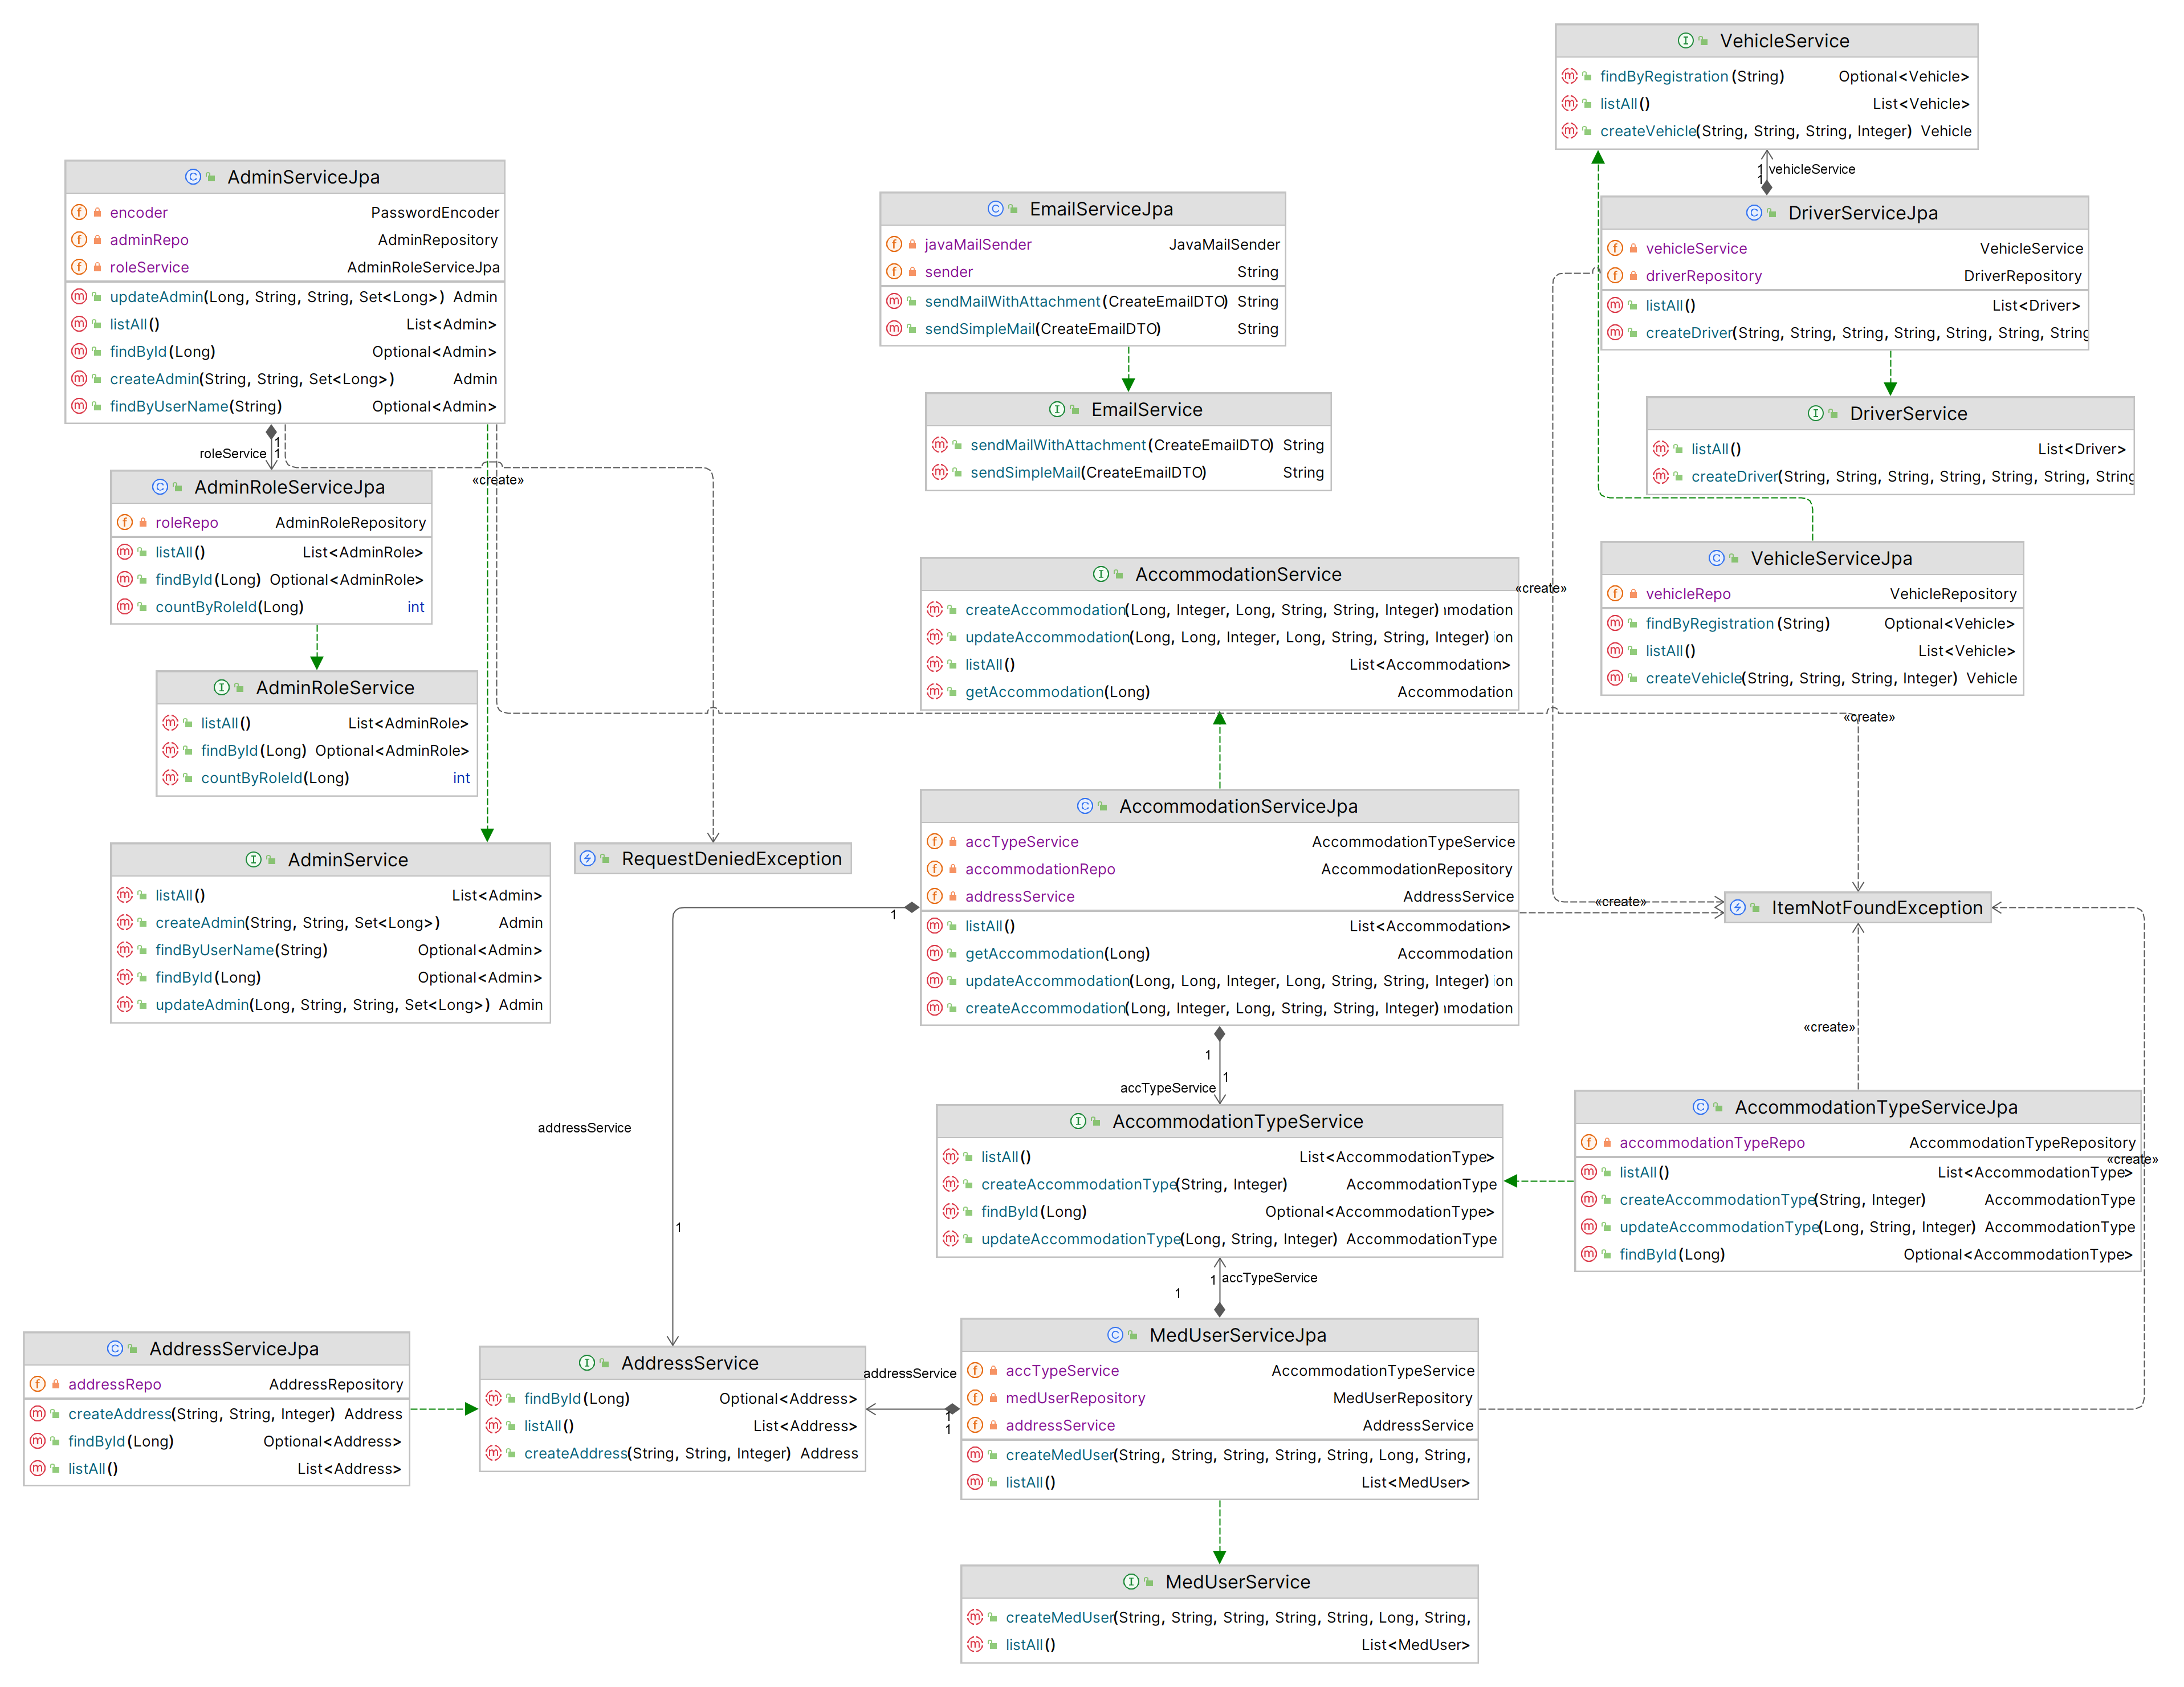
\includegraphics[width=\textwidth]{slike/service.PNG}
				\caption{Dijagram razreda - Service}
				\label{serviceDiagram}
			\end{figure}
			
			{Navedene \textit{Service} klase su \textit{Spring Service} klase, sadrže poslovnu logiku aplikacije, tj. odgovorni su za obradu podataka, implementaciju algoritama itd. Ponašaju se kao sloj između \textit{Controllera} i \textit{Repositoryja}.\\
			\textit{AdminService} sadrži metodu \textit{createAdmin} za stvaranje administratora. Postoji provjera raznih svojstava, poput duljine lozinke, duljine nadimka, postoji li već neki administrator s tim nadimkom, postojanje navedenih uloga itd. Ako je sve uspješno sprema se novi administrator u \textit{AdminRepository}.}\\
			
			\begin{figure}[H]
				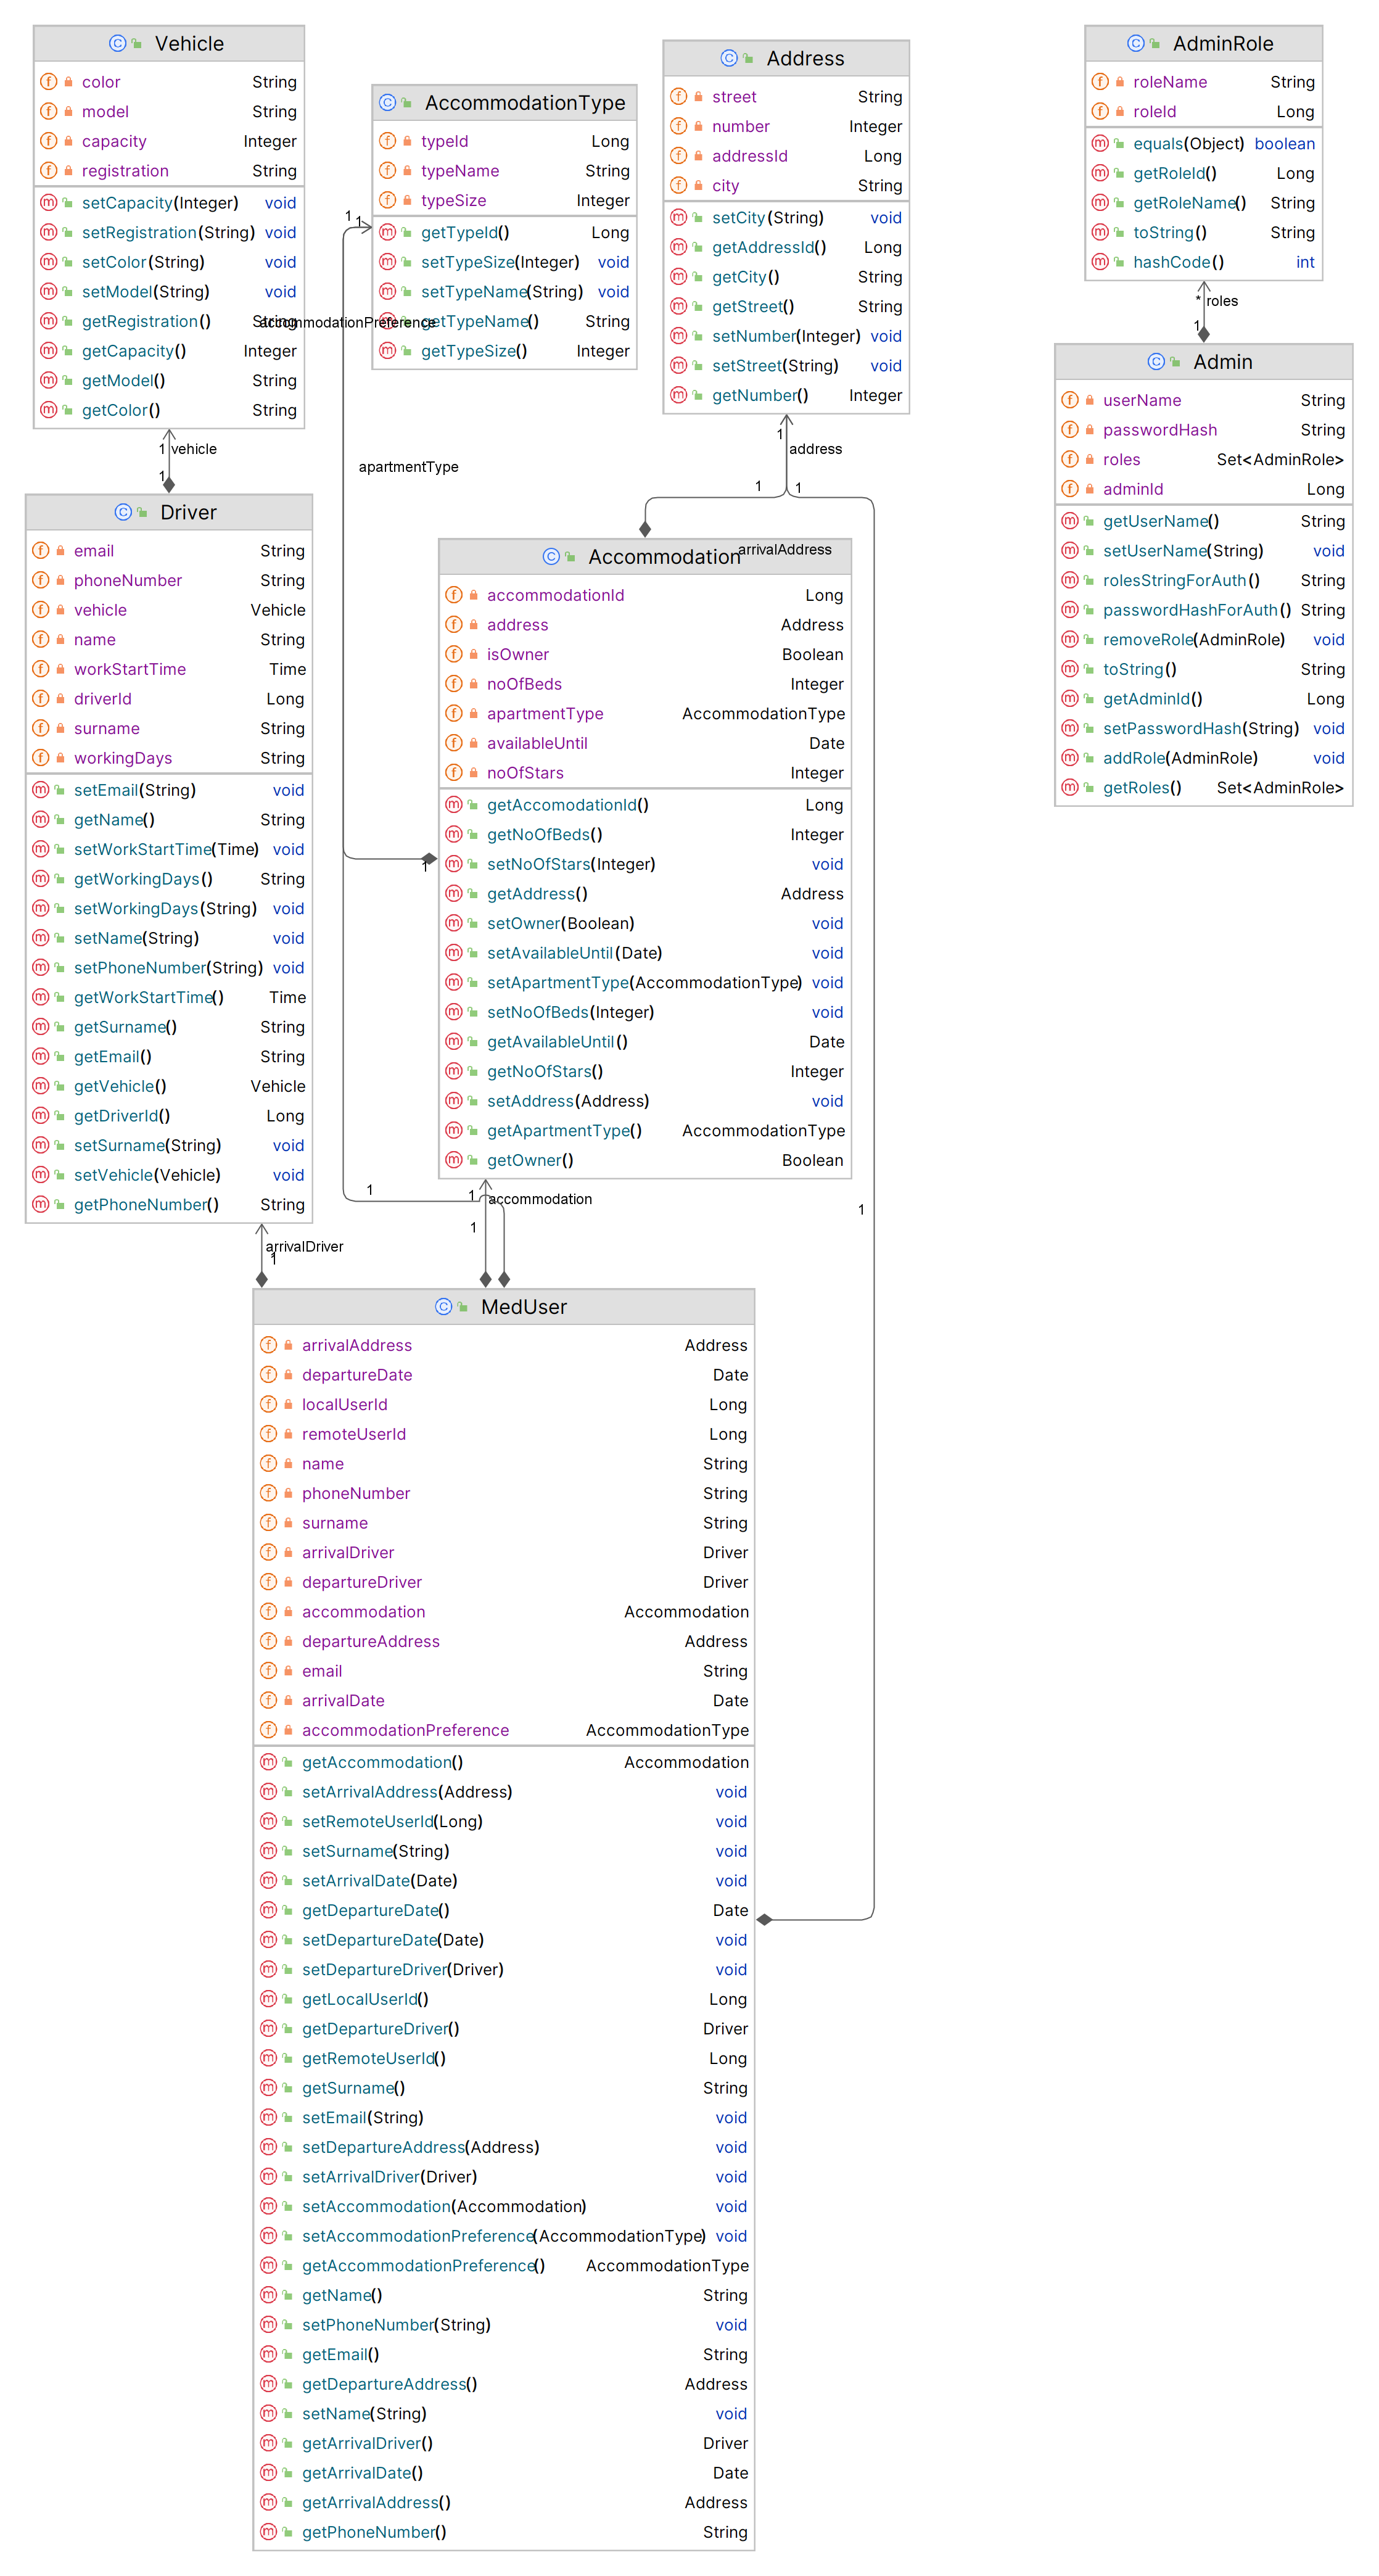
\includegraphics[width=\textwidth]{slike/domain.PNG}
				\caption{Dijagram razreda - Models}
				\label{domainDiagram}
			\end{figure}
			
			{Modeli predstavljaju strukturu baze podataka u našoj aplikaciji. Tako imamo klase: \textit{Admin, MedUser, Accomomodation te Transport} sa svojim privatnim atributima te javnim metodama. Tako na primjer \textit{Admin} ima svoj ID, nadimak, ime te pripadajuće uloge, koje mogu biti smještajni administrator(ima najveće ovlasti), korisnički administrator te prijevozni administrator, što je sadržano u enumeraciji \textit{AdminRole}. \textit{Accommodation} i \textit{Transport} sadrže sve podatke vezane uz smještaj, odnosno prijevoz, a \textit{MedUser} sadrži sve potrebno za definiranje korisnika medicinskih usluga. }\\
			
			
			
			%\textbf{\textit{dio 2. revizije}}\\			
			
			%\textit{Prilikom druge predaje projekta dijagram razreda i opisi moraju odgovarati stvarnom stanju implementacije}
			
			
			
			\eject
		
		\section{Dijagram stanja}
			
			{Na slici 4.7 prikazan je dijagram stanja. Prvo na što admin naiđe je prijava, te nakon toga mu se prikaže web stranica za admina. Na toj stranici može odabrati opciju pregleda svih unesenih podataka te izbrisati ili promijeniti iste. Ako je admin prijavljen kao korisnički admin onda on odabirom opcije za 
			dodavanje novog korisnika može dodati novog korisnika. Dok ako je admin prijavljen kao admin prijevoza, može dodavati nove prijevoznike. Smještajni admin može odabirom opcije za dodavanje novog administratora, dodati novog administratora, ali isto tako odabirom opcije za dodavanje novog smještaja, može dodati novi smještaj.  }
			
			\begin{figure}[H]
				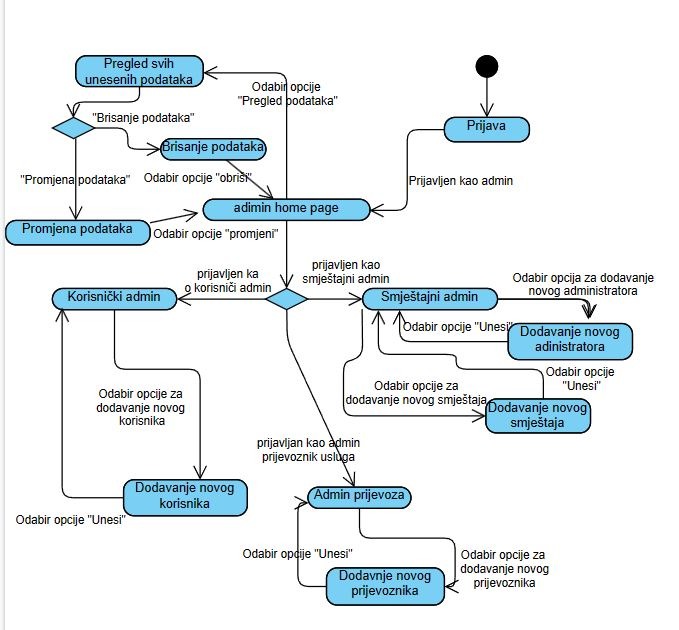
\includegraphics[width=\linewidth]{slike/Dijagram stanja.JPG}
				\centering
				\caption{Dijagram stanja}
				\label{fig:Dijagram stanja}
			\end{figure}

			%\textbf{\textit{dio 2. revizije}}\\
			
			%\textit{Potrebno je priložiti dijagram stanja i opisati ga. Dovoljan je jedan dijagram stanja koji prikazuje \textbf{značajan dio funkcionalnosti} sustava. Na primjer, stanja korisničkog sučelja i tijek korištenja neke ključne funkcionalnosti jesu značajan dio sustava, a registracija i prijava nisu. }
			
			
			\eject 
		
		\section{Dijagram aktivnosti}

		{Na slici 4.8 prikaza je dijagram aktivnosti. Sve počinje prijavom. Uneseno korisničko ime i lozinka se provjeravaju s bazom podataka. Ako je neispravna prijava, admin se vrača na obrazac za unos podataka za prijavu, dok ako je prijava uspješna, pojavljuje se prikaz vrsta admina.
		Ako je prijavljen korisnički admin, on može dodavati nove korisnike. Adim prijevoza može dodavati nove prijevoznike. Dok smještajni admin može dodavati novi smještaj te dodavati nove admine.}
			
		\begin{figure}[H]
			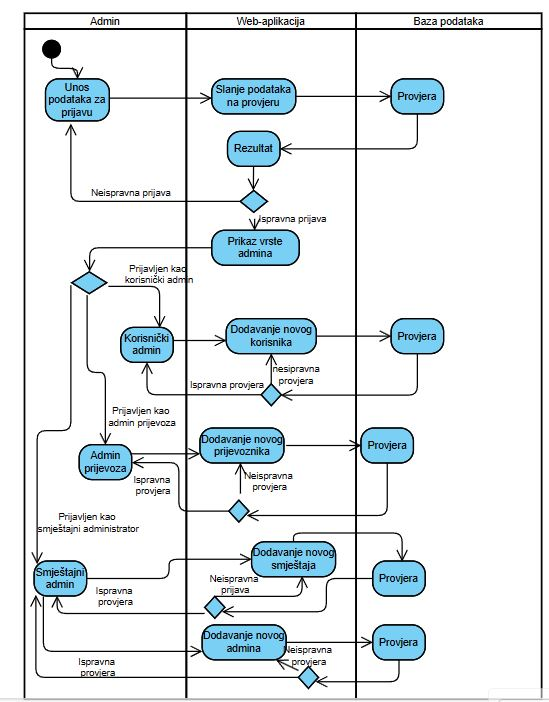
\includegraphics[width=\linewidth]{slike/Dijagram aktivnsti.JPG}
			\centering
			\caption{Dijagram aktivnosti}
			\label{fig:Dijagram aktivnosti}
		\end{figure}


			%\textbf{\textit{dio 2. revizije}}\\
			
			 %\textit{Potrebno je priložiti dijagram aktivnosti s pripadajućim opisom. Dijagram aktivnosti treba prikazivati značajan dio sustava.}
			
			\eject
		\section{Dijagram komponenti}

		{Na slici 4.9 prikazan je dijagram komponenti koji pokazuje međuovisnosti između frontenda, backenda i baze podataka. Frontend ima poseban server za HTML, CSS i JS datoteke koje služe za strukturu i dizajn web stranice. REST API komponenti pristupa se preko sučelja za dohvat JSON podataka te poslužuje podatke backendu. 
		Cijeli backend je napravljen na Springu te backend komunicira s bazom podataka slanjem SQL upita.}
		
			\begin{figure}[H]
				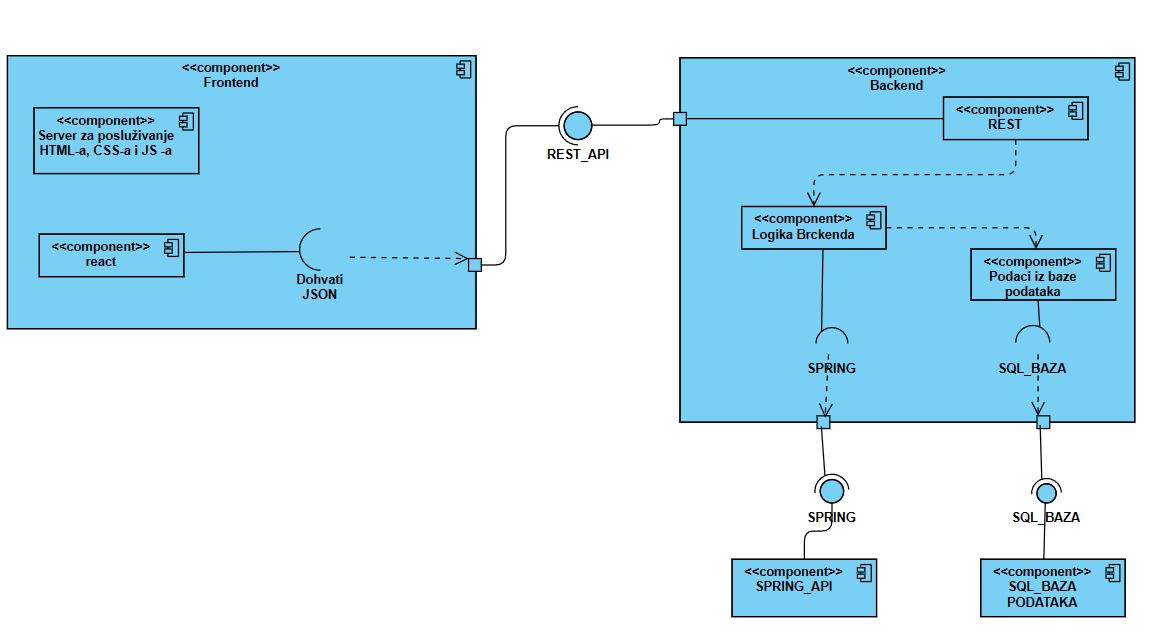
\includegraphics[width=\linewidth]{slike/dijagram komponenti.JPG}
				\centering
				\caption{Dijagram komponenti}
				\label{fig:Dijagram komponenti}
			\end{figure}			%\textbf{\textit{dio 2. revizije}}\\
		
			 %\textit{Potrebno je priložiti dijagram komponenti s pripadajućim opisom. Dijagram komponenti treba prikazivati strukturu cijele aplikacije.}
	\chapter{Implementacija i korisničko sučelje}
		
		
		\section{Korištene tehnologije i alati}
		
			%\textbf{\textit{dio 2. revizije}}
			
			 %\textit{Detaljno navesti sve tehnologije i alate koji su primijenjeni pri izradi dokumentacije i aplikacije. Ukratko ih opisati, te navesti njihovo značenje i mjesto primjene. Za svaki navedeni alat i tehnologiju je potrebno \textbf{navesti internet poveznicu} gdje se mogu preuzeti ili više saznati o njima}.
			\eject 
			Tehnologije i alati koji su se koristili u izradi aplikaciji grupirane su s obzirom na mjseto primjene: backend, frontend, baza podataka, dokumentacija i ispitivanje.
			
			\textbf{Backend}
			Korišteno je radno okruženje InteliJ IDEA koje je razvila tvrtka JetBrains za koji postoji komercijalna, Apache 2 licensa, a radno okruženje se koristilo preko fakultetskog računa. 
			Za frontend
	
		\section{Ispitivanje programskog rješenja}
			
			%\textbf{\textit{dio 2. revizije}}\\
			
			 %\textit{U ovom poglavlju je potrebno opisati provedbu ispitivanja implementiranih funkcionalnosti na razini komponenti i na razini cijelog sustava s prikazom odabranih ispitnih slučajeva. Studenti trebaju ispitati temeljnu funkcionalnost i rubne uvjete.}
	
			
			%\subsection{Ispitivanje komponenti}
			%\textit{Potrebno je provesti ispitivanje jedinica (engl. unit testing) nad razredima koji implementiraju temeljne funkcionalnosti. Razraditi \textbf{minimalno 6 ispitnih slučajeva} u kojima će se ispitati redovni slučajevi, rubni uvjeti te izazivanje pogreške (engl. exception throwing). Poželjno je stvoriti i ispitni slučaj koji koristi funkcionalnosti koje nisu implementirane. Potrebno je priložiti izvorni kôd svih ispitnih slučajeva te prikaz rezultata izvođenja ispita u razvojnom okruženju (prolaz/pad ispita). }
			
			
			
			%\subsection{Ispitivanje sustava}
			
			 %\textit{Potrebno je provesti i opisati ispitivanje sustava koristeći radni okvir Selenium\footnote{\url{https://www.seleniumhq.org/}}. Razraditi \textbf{minimalno 4 ispitna slučaja} u kojima će se ispitati redovni slučajevi, rubni uvjeti te poziv funkcionalnosti koja nije implementirana/izaziva pogrešku kako bi se vidjelo na koji način sustav reagira kada nešto nije u potpunosti ostvareno. Ispitni slučaj se treba sastojati od ulaza (npr. korisničko ime i lozinka), očekivanog izlaza ili rezultata, koraka ispitivanja i dobivenog izlaza ili rezultata.\\ }
			 
			 %\textit{Izradu ispitnih slučajeva pomoću radnog okvira Selenium moguće je provesti pomoću jednog od sljedeća dva alata:}
			 %\begin{itemize}
			 %	\item \textit{dodatak za preglednik \textbf{Selenium IDE} - snimanje korisnikovih akcija radi automatskog ponavljanja ispita	}
			 %	\item \textit{\textbf{Selenium WebDriver} - podrška za pisanje ispita u jezicima Java, C\#, PHP koristeći posebno programsko sučelje.}
			 %\end{itemize}
		 	%\textit{Detalji o korištenju alata Selenium bit će prikazani na posebnom predavanju tijekom semestra.}
			
			\eject 
		
		
		\section{Dijagram razmještaja}
			
			%\textbf{\textit{dio 2. revizije}}
			
			 %\textit{Potrebno je umetnuti \textbf{specifikacijski} dijagram razmještaja i opisati ga. Moguće je umjesto specifikacijskog dijagrama razmještaja umetnuti dijagram razmještaja instanci, pod uvjetom da taj dijagram bolje opisuje neki važniji dio sustava.}
			
			\eject 
		
		\section{Upute za puštanje u pogon}
		
			%\textbf{\textit{dio 2. revizije}}\\
		
			 %\textit{U ovom poglavlju potrebno je dati upute za puštanje u pogon (engl. deployment) ostvarene aplikacije. Na primjer, za web aplikacije, opisati postupak kojim se od izvornog kôda dolazi do potpuno postavljene baze podataka i poslužitelja koji odgovara na upite korisnika. Za mobilnu aplikaciju, postupak kojim se aplikacija izgradi, te postavi na neku od trgovina. Za stolnu (engl. desktop) aplikaciju, postupak kojim se aplikacija instalira na računalo. Ukoliko mobilne i stolne aplikacije komuniciraju s poslužiteljem i/ili bazom podataka, opisati i postupak njihovog postavljanja. Pri izradi uputa preporučuje se \textbf{naglasiti korake instalacije uporabom natuknica} te koristiti što je više moguće \textbf{slike ekrana} (engl. screenshots) kako bi upute bile jasne i jednostavne za slijediti.}
			
			
			 %\textit{Dovršenu aplikaciju potrebno je pokrenuti na javno dostupnom poslužitelju. Studentima se preporuča korištenje neke od sljedećih besplatnih usluga: \href{https://aws.amazon.com/}{Amazon AWS}, \href{https://azure.microsoft.com/en-us/}{Microsoft Azure} ili \href{https://www.heroku.com/}{Heroku}. Mobilne aplikacije trebaju biti objavljene na F-Droid, Google Play ili Amazon App trgovini.}
			
			
			\eject 
	\chapter{Zaključak i budući rad}
		
		\textbf{\textit{dio 2. revizije}}\\
		
		 \textit{U ovom poglavlju potrebno je napisati osvrt na vrijeme izrade projektnog zadatka, koji su tehnički izazovi prepoznati, jesu li riješeni ili kako bi mogli biti riješeni, koja su znanja stečena pri izradi projekta, koja bi znanja bila posebno potrebna za brže i kvalitetnije ostvarenje projekta i koje bi bile perspektive za nastavak rada u projektnoj grupi.}
		
		 \textit{Potrebno je točno popisati funkcionalnosti koje nisu implementirane u ostvarenoj aplikaciji.}
		
		\eject 
	\chapter*{Popis literature}
		\addcontentsline{toc}{chapter}{Popis literature}
	 	
 		%\textbf{\textit{Kontinuirano osvježavanje}}
	
		%\textit{Popisati sve reference i literaturu koja je pomogla pri ostvarivanju projekta.}
		
		
		\begin{enumerate}
			
			
			\item  Programsko inženjerstvo, FER ZEMRIS, \url{http://www.fer.hr/predmet/proinz}
			
			\item  Learn Spring Boot, \url{https://www.baeldung.com/spring-boot}
			
			\item  Astah Community, \url{http://astah.net/editions/uml-new}
			
			\item  Visual Paradigm Online, \url{https://online.visual-paradigm.com/}
			
			\item  Upute za deploy na Render, \url{https://github.com/progi-devops}
			
			\item  Stack overflow, \url{https://stackoverflow.com/}
			
			\item  React reference overview, \url{https://react.dev/reference/react}
			
			\item  Get started with Bootstrap, \url{https://getbootstrap.com/docs/5.3/getting-started/introduction/}
			
			\item  Java Networking, \url{https://docs.oracle.com/javase/8/docs/technotes/guides/}
			
			\item  Render, \url{https://render.com/}
			
		\end{enumerate}
		
		 
	
	
	\begingroup
	\renewcommand*\listfigurename{Indeks slika i dijagrama}
	%\renewcommand*\listtablename{Indeks tablica}
	%\let\clearpage\relax
	\listoffigures
	%\vspace{10mm}
	%\listoftables
	\endgroup
	\addcontentsline{toc}{chapter}{Indeks slika i dijagrama}


	
	\eject 
		
	\chapter*{Dodatak: Prikaz aktivnosti grupe}
		\addcontentsline{toc}{chapter}{Dodatak: Prikaz aktivnosti grupe}
		
		\section*{Dnevnik sastajanja}
		
		%\textbf{\textit{Kontinuirano osvježavanje}}\\
		
		 %\textit{U ovom dijelu potrebno je redovito osvježavati dnevnik sastajanja prema predlošku.}
		
		\begin{packed_enum}
			\item  sastanak
			
			\item[] \begin{packed_item}
				\item Datum: 18. listopada 2023.
				\item Prisustvovali: T. Pranjić, J. Mihelčić, A. Mesić, D. Mišetić, A. Sorić, I. Ćorluka, N. Perić
				\item Teme sastanka:
				\begin{packed_item}
					\item Formiranje tima
					\item Odabir voditelja
				\end{packed_item}
			\end{packed_item}
			
			\item  sastanak
			\item[] \begin{packed_item}
				\item Datum: 25. listopada 2023.
				\item Prisustvovali: T. Pranjić, J. Mihelčić, A. Mesić, D. Mišetić, A. Sorić, I. Ćorluka, N. Perić
				\item Teme sastanka:
				\begin{packed_item}
					\item  Razjašnjavanje pojedinosti oko projektnog zadatka

				\end{packed_item}
			\end{packed_item}
      
      \item  sastanak
			\item[] \begin{packed_item}
			  \item Datum: 25. listopada 2023.
				\item Prisustvovali: A. Sorić, D. Mišetić
				\item Teme sastanka:
				\begin{packed_item}
					\item  Opis projektnog zadatka
        \end{packed_item}
     \end{packed_item}
			
	  \item  sastanak
			\item[] \begin{packed_item}
			  \item Datum: 08. siječnja 2024.
				\item Prisustvovali:  T. Pranjić, J. Mihelčić, A. Mesić, D. Mišetić, A. Sorić, I. Ćorluka, N. Perić
				\item Teme sastanka:
				\begin{packed_item}
					\item  Plan rada za drugi ciklus
        \end{packed_item}
	\end{packed_item}

		%
 
		\end{packed_enum}
		
		\eject
		\section*{Tablica aktivnosti}
		
			%\textbf{\textit{Kontinuirano osvježavanje}}\\
			
			 %\textit{Napomena: Doprinose u aktivnostima treba navesti u satima po članovima grupe po aktivnosti.}

			\begin{longtblr}[
					label=none,
				]{
					vlines,hlines,
					width = \textwidth,
					colspec={X[7, l]X[1, c]X[1, c]X[1, c]X[1, c]X[1, c]X[1, c]X[1, c]}, 
					vline{1} = {1}{text=\clap{}},
					hline{1} = {1}{text=\clap{}},
					rowhead = 1,
				} 
			
\SetCell[c=1]{c}{} & \SetCell[c=1]{c}{\rotatebox{90}{\textbf{Tomislav Pranjić}}} & \SetCell[c=1]{c}{\rotatebox{90}{\textbf{Ante Sorić}}} &	\SetCell[c=1]{c}{\rotatebox{90}{\textbf{Diego Mišetić}}} & \SetCell[c=1]{c}{\rotatebox{90}{\textbf{Josip Mihelčić}}} &	\SetCell[c=1]{c}{\rotatebox{90}{\textbf{Antonia Mesić}}} & \SetCell[c=1]{c}{\rotatebox{90}{\textbf{Ivan Ćorluka}}} &	\SetCell[c=1]{c}{\rotatebox{90}{\textbf{Nikola Perić}}} \\  

         Upravljanje projektom 			            & 4 &  &  & 8 &  &  & \\ 
				Opis projektnog zadatka 	              &  & 8 & 8 &  &  &  & \\
				Funkcionalni zahtjevi       		          &  &  &  &  &  &  & 8 \\ 
				Opis pojedinih obrazaca 		          & 1 &  &  & 2 &  &  &  \\ 
				Dijagram obrazaca 				             & 3 &  &  & 3 &  &  &  \\ 
				Sekvencijski dijagrami 				        &  &  & 5 &  &  &  &  \\ 
				Opis ostalih zahtjeva 				          &  &  &  &  &  &  &  \\ 
				Arhitektura i dizajn sustava	          & 2 &  &  &  &  &  & 1  \\ 
				Baza podataka						  			& 3 &  & 3 &  &  &  &   \\ 
				Dijagram razreda 					 		   &  & 4 &  & 2 &  &  &   \\  
				Dijagram stanja						   	         &  &  & 4 &  &  &  &  \\ 
				Dijagram aktivnosti 				  	      &  &  & 4 &  &  &  &  \\ 
				Dijagram komponenti				 	       &  &  & 4 &  &  &  &  \\ 
				Korištene tehnologije i alati 	 	       & 2 &  &  &  &  &  &  \\ 
				Ispitivanje programskog rješenja 	&  &  &  &  &  &  &  \\ 
				Dijagram razmještaja						&  &  & 4 &  &  &  &  \\ 
				Upute za puštanje u pogon 			   & 4 &  &  &  &  &  &  \\  
				Dnevnik sastajanja 			                  &  &  &  &  &  &  &  \\ 
				Zaključak i budući rad 		                 & 2 &  &  &  &  &  &  \\  
				Popis literature 								  &  &  &  &  &  &  &  \\  
				&  &  &  &  &  &  &  \\ \hline 
				\textit{Backend: Generičke funkcionalnosti i sigurnost} 			&  & 16 &  & 18 &  &  &  \\ 
				\textit{Frontend: Izrada početne stranice} 				&  &  &  &  &  &  &  \\
				\textit{Frontend: Izrada stranice za prijavu}             &  &  &  &  &  &  & 8 \\ 
				\textit{Baza podataka: Izrada baze podataka} 		 			&  &  &  &  &  &  & \\  
				\textit{Backend: Spajanje s bazom podataka} 							&  &  &  &  &  &  &  \\ 
				\textit{Puštanje sustava u pogon}							& 10 &  &  & 8 &  &  &\\ 
			\end{longtblr}
					
					
		\eject
		\section*{Dijagrami pregleda promjena}
		
		%\textbf{\textit{dio 2. revizije}}\\
		
		%\textit{Prenijeti dijagram pregleda promjena nad datotekama projekta. Potrebno je na kraju projekta generirane grafove s gitlaba prenijeti u ovo poglavlje dokumentacije. Dijagrami za vlastiti projekt se mogu preuzeti s gitlab.com stranice, u izborniku Repository, pritiskom na stavku Contributors.}
		
	



\end{document} %naredbe i tekst nakon ove naredbe ne ulaze u izgrađen dokument 


